\documentclass[11pt,a4paper]{article}

\usepackage{kotex}
\usepackage[margin=1in]{geometry}
\usepackage{booktabs}
\usepackage{listings}
\usepackage{xcolor}
\usepackage{hyperref}
\usepackage{graphicx}
\graphicspath{{../figures/}{figures/}}

\lstset{
  basicstyle=\ttfamily\small,
  breaklines=true,
  frame=single,
  columns=fullflexible,
  keepspaces=true,
}

\title{OpenMP Performance Exploration\\Analyzing Naive Prime Search}
\author{2024404060 강민혁}
\date{\today}

\begin{document}
\maketitle

\section{Experimental Environment}

\subsection{Hardware}

\begin{table}[h]
\centering
\begin{tabular}{ll}
\toprule
구성 요소 & 사양 \\
\midrule
CPU & AMD Ryzen 9 5900X \\
코어 / 논리 스레드 & 12 cores / 12 threads (SMT-off), 24 threads (SMT-on) \\
CCD 구성 & 2 CCDs $\times$ 6 cores per CCD \\
아키텍처 & x86-64 \\
CPU 클럭 & 4.5 GHz 고정 (PBO disabled) \\
\bottomrule
\end{tabular}
\caption{시스템 하드웨어 스펙}
\end{table}

AMD Ryzen 9 5900X는 6코어로 구성된 두 개의 Core Complex Die(CCD)를 갖는 구조이며, Intel의 Hyper-Threading에 해당하는 Simultaneous Multi-Threading(SMT) 기능은 UEFI 레벨에서 활성화 및 비활성화한 두 조건으로 각각 실험하였다. SMT-off에서는 12개 물리 코어와 12개 논리 스레드를 사용하고, SMT-on에서는 12개 물리 코어와 24개 논리 스레드를 사용한다. 본 실험에서는 CCD와 관련하여 intra-CCD 영역과 cross-CCD 영역에서의 스케일링 특성을 비교하였다.

\subsection{Cache Hierarchy}

AMD Ryzen 9 5900X(Zen 3)의 캐시 계층은 표 \ref{tab:cache}와 같으며, 모든 계층의 캐시 라인 크기는 64\,B로 동일하다~\cite{amd-ppr-family19h}. 

\footnote{Ryzen 9 5900X가 속한 Family 19h Model 21h의 공식 PPR 문서를 찾을 수 없어 본 실험에서는 동일한 Zen 3 아키텍처를 공유하는 Family 19h Model 51h의 공식 문서에 기술되어있는 캐시 정보를 바탕으로 진행하였다.}.

\begin{table}[h]
\centering
\begin{tabular}{lllll}
\toprule
계층 & 용량 (코어/CCD당) & 총 용량 & 구조 & 공유 범위 \\
\midrule
L1I & 32\,KiB & 384\,KiB & 8-way set assoc. & 코어 전용 \\
L1D & 32\,KiB & 384\,KiB & 8-way set assoc. & 코어 전용 \\
L2  & 512\,KiB & 6\,MiB & 8-way set assoc. & 코어 전용 (inclusive) \\
L3  & 32\,MiB / CCD & 64\,MiB & 16-way set assoc. & CCD 내 6코어 공유 (victim) \\
\bottomrule
\end{tabular}
\caption{AMD Ryzen 9 5900X (Zen 3) 캐시 계층}
\label{tab:cache}
\end{table}

L1 캐시는 코어당 64\,KiB(32\,KiB L1I + 32\,KiB L1D)이다. L2 캐시는 코어 전용 512\,KiB 캐시로, L1에 대해 inclusive하게 동작하며 L1 miss를 처리한다.

L3 캐시는 CCD 내 6개 코어가 공유하는 32\,MiB 캐시로, 5900X 전체로는 64\,MiB(2 CCDs)에 해당한다. L3는 non-inclusive하게 동작하며, 일반적으로 L2의 victim cache의 역할을 수행한다. 과제의 범위에는 벗어나지만, 캐시 관련 실험까지 진행하여 표~\ref{tab:cache}의 계층 구조를 기준으로 L1/L2/L3 용량 경계와 CCD 단위 공유 여부까지 해석하고자 한다.

\subsection{SMT 모드의 캐시 측면 영향}

본 실험에서는 UEFI 설정을 통해 SMT를 비활성화한 조건과 활성화한 조건을 모두 측정하였다. 두 조건에서 각각 실험 별로 동일한 탐색 공간을 사용하되, 결과 파일을 분리하였다.

\paragraph{스레드당 캐시 자원 독점 사용.}
SMT가 활성화된 상태에서는 두 개의 논리 스레드가 하나의 물리 코어에 속한 L1/L2 캐시를 competitive sharing해야 하므로, 두 스레드가 교차 실행되며 L1 캐시 내용에 thrashing이 발생할 수 있다. SMT-off를 하면 각 OpenMP 스레드는 해당 코어의 L1(64\,KiB; L1I 32\,KiB + L1D 32\,KiB) 및 L2(512\,KiB)를 100\,\% 점유하기에, 스레드 간 캐시 competition이 사라지고 L1 적중률이 극대화되며 접근 지연 시간 또한 일정해질 것이다. 이는 동일 조건의 반복 측정에서 분산을 줄여 측정 신뢰도를 높이는 효과도 가질 것이다.

\paragraph{스레드당 실효 L3 working set의 증가.}
SMT-on에서는 하나의 CCD에서 12개의 논리 스레드가 32\,MiB의 L3를 공유하므로 스레드당 약 2.66\,MiB을 점유 가능 반면, SMT-off에서는 6개의 물리 스레드만이 동일한 32\,MiB를 공유하기에 스레드당 약 5.33\,MiB를 점유할 수 있다. 즉, SMT-off에서는 working set이 L2를 넘는 경우에도 capacity miss가 줄어든다.

\subsection{Software}

\begin{table}[h]
\centering
\begin{tabular}{ll}
\toprule
구성 요소 & 버전 \\
\midrule
운영체제 & Arch Linux \\
커널 & Linux 6.19.14-arch1-1 \\
컴파일러 & GCC 15.2.1 (20260209) \\
컴파일 옵션 & \texttt{-O3 -march=native -fopenmp -Wall -Wextra} \\
\bottomrule
\end{tabular}
\caption{소프트웨어 환경}
\end{table}

\texttt{-march=native}는 Zen 3가 제공하는 instruction과 마이크로아키텍처별 코드 생성을 활용하기 위하여 선택하였다. 물론 다른 환경에서의 재현성은 낮추지만, 본 과제에서 사용 가능한 컴퓨팅 자원과 시간 자원의 한계가 있으며, 또한, 단일 시스템 내에서 스레드 수, 스케줄링, 스레드 배치/고정 등 상대적 영향을 비교하는 것이 목적이기에 사용하였다.

\section{Experimental Design}

본 과제의 목적은 OpenMP를 활용해 naive prime search algorithm을 병렬화하고, 다양한 설정 및 런타임 매개변수가 하드웨어 실행 효율성에 미치는 영향을 심층적으로 분석하는 것이다. 실험에서는 단일 OpenMP 커널에서 병렬화 방식, 스케줄링 정책, 스레드 배치/고정, 런타임 대기 정책이 성능에 미치는 영향을 분리하여 정량화하고, 분석하는 것을 목표로 하였다. 이에 더해, CCD 경계와 캐시 계층의 영향을 별도로 관찰하기 위해 pointer chase 기반 캐시 실험과 false sharing 실험을 추가하였다. 실험은 \texttt{run\_experiments.py}가 모든 실험 각각에 맞는 탐색 공간을 순차적으로 실행하는 방식으로 구성하였으며, 각 조합은 \texttt{grid\_search.py}에서 OpenMP 환경 변수와 실행 인자 등으로 변경되어 C로 작성된 OpenMP 환경에서 실행된다. \texttt{run\_experiments.py}와 \texttt{grid\_search.py}의 주요 클래스 및 함수는 부록~\ref{app:code}에 수록한다.

\subsection{SMT 모드별 실행과 CPU 배치 통제}

SMT는 UEFI에서 수동으로 설정하였으며, SMT-off와 SMT-on에 따른 실험 결과는 별도로 저장하였다. 각 실험은 두 SMT 모드 모두에서 동일한 탐색 공간을 사용한다. 단, 논리 코어 해석과 일부 결과 해석은 SMT 모드에 따라 달라진다.

SMT-on에서 논리 코어 \texttt{0-11}은 12개 물리 코어의 첫 번째 hardware thread이고, \texttt{12-23}은 각 코어의 SMT sibling이다. 또한 \texttt{0-5}와 \texttt{12-17}은 첫 번째 CCD, \texttt{6-11}과 \texttt{18-23}은 두 번째 CCD에 속한다. 이 topology를 기준으로, 프로세스에 허용할 CPU 코어를 auto로 두는 경우는  표~\ref{tab:smt-affinity-summary}퍼럼 해석하였다. 반면 실험 F, H, I, J처럼 CCD 또는 물리 코어 배치 자체가 비교 대상인 경우에는 SMT-on에서도 설정 파일에 적어 둔 CPU 번호 목록을 그대로 적용하였다.

\begin{table}[h]
\centering
\begin{tabular}{cllp{0.32\linewidth}}
\toprule
\texttt{num\_threads} & 적용 대상 & SMT-off CPU set & SMT-on CPU set \\
\midrule
\texttt{1}  & 기본 매핑 & \texttt{0}    & \texttt{0} \\
\texttt{2}  & 기본 매핑 & \texttt{0-1}  & \texttt{0-1} \\
\texttt{4}  & 기본 매핑 & \texttt{0-3}  & \texttt{0-3} \\
\texttt{6}  & 기본 매핑 & \texttt{0-5}  & \texttt{0-5} \\
\texttt{8}  & 기본 매핑 & \texttt{0-7}  & \texttt{0-7} \\
\texttt{12} & 기본/G 매핑 & \texttt{0-11} & \texttt{0-11} \\
\texttt{16} & 기본 매핑 & \texttt{0-11} & \texttt{0-11,12-13,18-19} \\
\texttt{24} & 기본/G 매핑 & \texttt{0-11} & \texttt{0-23} \\
\bottomrule
\end{tabular}
\caption{CPU set auto 선택 시 SMT 모드별 CPU 배치 해석}
\label{tab:smt-affinity-summary}
\end{table}

\subsection{공통 벤치마크 및 계측 방법}

실험 A--D 및 H는 동일한 naive prime search 커널을 사용한다. 각 커널은 후보 정수 $2,\ldots,\texttt{limit}$에 대해 trial division 기반 검사를 수행한다.

\begin{lstlisting}[language=C]
static bool is_prime(uint64_t n) {
    if (n < 2) return false;
    if (n == 2) return true;
    if ((n & 1u) == 0) return false;

    for (uint64_t d = 3; d <= n / d; d += 2) {
        if (n % d == 0) return false;
    }
    return true;
}
\end{lstlisting}

실험 E--G 및 I는 pointer chase 기반 메모리 접근 부하를 사용하여 캐시 용량 경계, CCD 간 L3 공유, 스레드 배치/고정에 따른 private L1/L2 지역성을 분리해 관찰한다. 실험 J는 false sharing을 의도적으로 유발한 조건과 padding으로 제거한 조건을 비교한다.

각 실행에서는 스레드 풀 생성 비용, fork--join 비용, 직렬 실행 시간, 병렬 실행 시간을 분리해 기록하였다. 직렬 및 병렬 커널은 각각 세 번 반복한 값 중 최솟값을 채택하여 os interrupt 등으로 인한 노이즈를 줄이고자 하였다. 최종 결과로, 요청한 스레드 수와 실제 OpenMP 스레드 수, fork--join 오버헤드를 포함한 speedup과 이를 제외한 오버헤드 제외 speedup(pure speedup), wall-clock 실행 시간과 실행 상태도 함께 저장하였다.

\texttt{limit} 후보는 별도의 사전 실험으로 정하였다. 실험에 사용하는 naive prime search과 같은 커널에서 1000단위로 증가시키며, $10^3$부터 $10^8$까지 실행 시간을 측정하였다. 싱글 코어/스레드로 측정하였다. limit이 작을 때에는 수십 $\mu$s 수준으로 측정 오버헤드의 영향을 크게 받는 반면 \texttt{limit}이 커질수록 ms--s 단위의 안정적인 시간 구간에 진입함을 확인하였다. 이때, $10^8$ 이상부터는 실험을 진행하기 어려울 정도로 연산 시간이 오래 걸렸다. 이를 바탕으로 실험 A와 D에서는 $10^3$부터 $10^7$까지의 로그 스케일 \texttt{limit}을 사용하여 오버헤드 지배 구간과 충분히 큰 계산 구간을 함께 포함시켰고, 실험 B, C, H에서는 $10^7$을 고정값으로 사용하였다.

\begin{figure}[h]
\centering
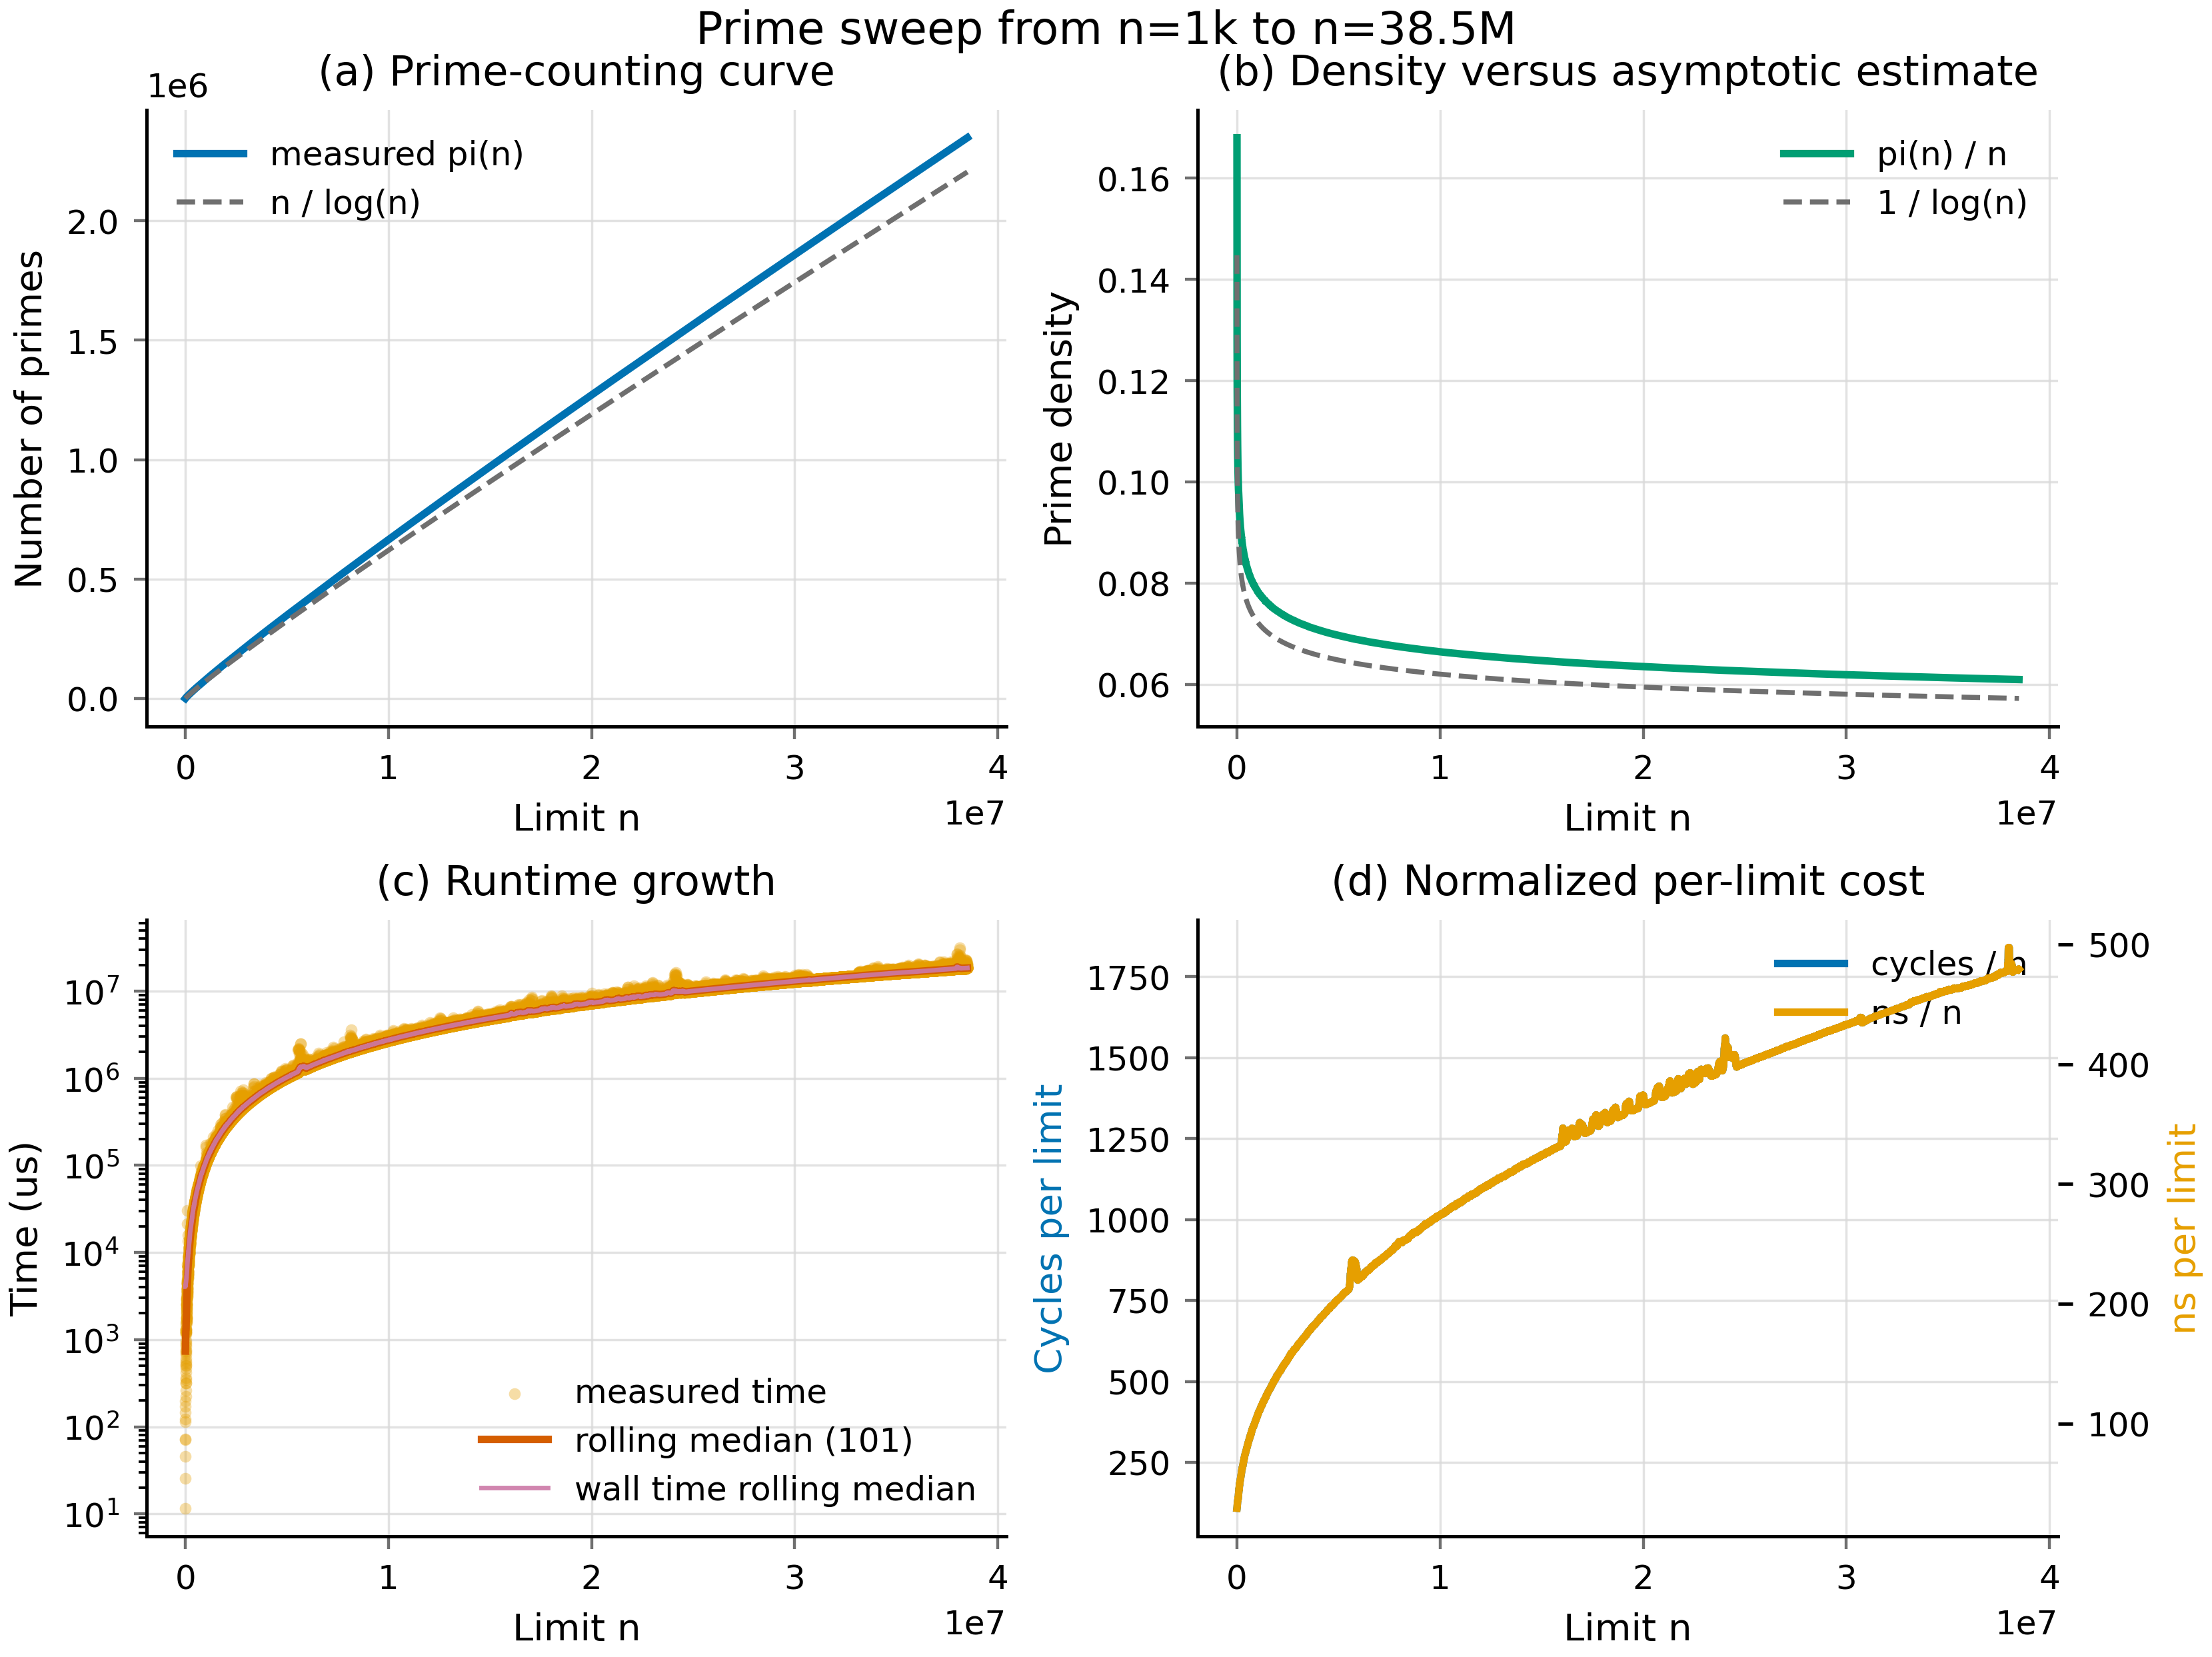
\includegraphics[width=0.95\linewidth]{figure_prime_range.png}
\caption{Naive prime search 실행 시간의 \texttt{limit}별 사전 측정 결과}
\label{fig:prime-range}
\end{figure}

이때, cycle이 deterministic하지 않다는 것을 확인하였다. 다만, 추세는 분명하기에 최대한 파이프라인을 직렬화하여 측정 오차를 줄이는 방식으로 실험을 설계하였다.

실험 조합은 생성 후 의미가 같은 설정을 정규화하여 중복 실행을 제거하였다. 정규화 기준과 실행 재현성 관련 구현은 뒤의 Grid Search 절에서 설명하며, 각 실험의 구체적인 탐색 공간은 Appendix~\ref{app:configs}에 설정 파일 전문을 수록하였다.

\subsection{Experiment A: Strong Scaling}

실험 A는 각 반복에서 OpenMP 병렬화 방식 자체는 바꾸지 않고, limit 크기와 스레드 수 변화가 스케일링에 어떤 영향을 주는지 측정한다. 이때, \texttt{parallel\_for}, \texttt{static, chunk=0}으로 유지하였다. 스레드 수는 CCD topology와 물리 코어 한계를 기준으로 선정하였다. \texttt{1}, \texttt{2}, \texttt{4}코어는 단일 CCD 내부의 intra-CCD 확장을, \texttt{6}코어는 single CCD boundary를, \texttt{8} 및 \texttt{12}코어는 두 CCD를 모두 사용하는 cross-CCD 확장과 전체 물리 코어까지의 scaling을 관찰하기 위한 지점이다. \texttt{16} 및 \texttt{24}스레드는 SMT-off에서는 oversubscription region이며, SMT-on에서는 추가 hardware thread를 사용하는 영역이다. 스레드 매핑은 물리 코어 기준, 근접 배치로 통일하였으며, 프로세스 레벨 CPU 배치는 표~\ref{tab:smt-affinity-summary}의 기본 매핑을 따른다.

\texttt{limit}이 작을 때, fork--join 및 scheduling 비용이 전체 실행 시간을 어느정도 차지하는가와, \texttt{limit}이 충분히 커지면 계산량이 오버헤드를 상쇄하며, 6코어 CCD 경계와 12개 물리 코어 포화점에서 pure speedup 곡선의 기울기 변화가 어느정도로 나타날 것인가를 파악하고자 한다.

\begin{table}[h]
\centering
\begin{tabular}{lp{0.70\linewidth}}
\toprule
설정 이름 & 값 \\
\midrule
\texttt{work\_sharing} & \texttt{parallel\_for} \\
\texttt{schedule\_kind} & \texttt{static} \\
\texttt{schedule\_chunk} & \texttt{0} \\
\texttt{task\_chunk\_size} & \texttt{0} \\
\texttt{num\_threads} & \texttt{1}, \texttt{2}, \texttt{4}, \texttt{6}, \texttt{8}, \texttt{12}, \texttt{16}, \texttt{24} \\
\texttt{proc\_bind} & \texttt{close} \\
\texttt{places} & \texttt{cores} \\
\texttt{wait\_policy} & \texttt{active} \\
\texttt{dynamic} & \texttt{false} \\
\texttt{limit} & $10^3$, $10^4$, $10^5$, $10^6$, $10^7$ \\
\bottomrule
\end{tabular}
\caption{실험 A의 파라미터 공간}
\end{table}

\subsection{Experiment B: Work Distribution and Scheduling}

실험 B는 고정된 limit과 물리 코어 수 조건에서 작업 분배 방식과 작업 분배 단위가 성능에 미치는 영향을 비교한다. 비교 대상은 \texttt{parallel\_for}, \texttt{manual}, \texttt{tasks}이다. 이 실험에서는 스레드 수, 스레드 배치/고정, 대기 정책, dynamic 스레드 조절 모두 고정하여, 관찰되는 차이가 작업 분배 방식과 chunk 크기에서 비롯되도록 통제하였다.

\begin{table}[h]
\centering
\begin{tabular}{lp{0.70\linewidth}}
\toprule
설정 이름 & 값 \\
\midrule
\texttt{work\_sharing} & \texttt{parallel\_for}, \texttt{manual}, \texttt{tasks} \\
\texttt{schedule\_kind} & \texttt{static}, \texttt{dynamic}, \texttt{guided}, \texttt{auto} \\
\texttt{schedule\_chunk} & \texttt{0}, \texttt{1}, \texttt{64}, \texttt{1024}, \texttt{16384}, \texttt{262144} \\
\texttt{task\_chunk\_size} & \texttt{0}, \texttt{256}, \texttt{8192}, \texttt{65536}, \texttt{524288} \\
\texttt{num\_threads} & \texttt{12} \\
\texttt{proc\_bind} & \texttt{close} \\
\texttt{places} & \texttt{cores} \\
\texttt{wait\_policy} & \texttt{active} \\
\texttt{dynamic} & \texttt{false} \\
\texttt{limit} & $10^7$ \\
\bottomrule
\end{tabular}
\caption{실험 B의 파라미터 공간}
\label{tab:expB-combos}
\end{table}

\texttt{manual}은 각 스레드가 연속 구간을 산술적으로 나누어 처리하므로
분배 오버헤드가 가장 작지만, naive prime search처럼 후보값이 커질수록
trial division 비용이 증가하는 커널에서는 구간별 부하 불균형에 취약할 수
있다. 반대로 \texttt{dynamic}, \texttt{guided}, \texttt{tasks}는 작업 큐 또는
태스크 생성 비용을 추가로 지불하는 대신 큰 후보가 몰리는 구간을 더 유연하게
분산한다. 따라서 이 실험은 naive prime search에서 정적 작업 분배 방식의 낮은 오버헤드와
동적 작업 분배 방식의 부하 균형 효과가 어느 지점에서 교차하는지, 그리고 동적 할당에서는 청크별로 어떠한 결과가 나오는지를 파악하고자 한다.

\subsection{Experiment C: Thread Placement and Pinning}

실험 C는 12개 물리 코어를 모두 사용하는 조건에서 스레드 배치/고정이 cross-CCD 실행에 미치는 영향을 분석한다. 스레드 수를 12개로 고정하면 SMT-off와 SMT-on 모두 첫 번째 hardware thread 중심의 물리 코어 배치가 기준이 되므로, 두 SMT 모드의 차이보다 스레드 배치/고정이 캐시 지역성, CCD 분산 등에 미치는 영향을 직접 비교할 수 있다. schedule은 실험 A의 기준 구성과 동일하게 유지하였다.

\begin{table}[h]
\centering
\begin{tabular}{lp{0.70\linewidth}}
\toprule
설정 이름 & 값 \\
\midrule
\texttt{work\_sharing} & \texttt{parallel\_for} \\
\texttt{schedule\_kind} & \texttt{static} \\
\texttt{schedule\_chunk} & \texttt{0} \\
\texttt{task\_chunk\_size} & \texttt{0} \\
\texttt{num\_threads} & \texttt{12} \\
\texttt{proc\_bind} & \texttt{false}, \texttt{close}, \texttt{spread} \\
\texttt{places} & \texttt{threads}, \texttt{cores} \\
\texttt{wait\_policy} & \texttt{active} \\
\texttt{dynamic} & \texttt{false} \\
\texttt{limit} & $10^7$ \\
\bottomrule
\end{tabular}
\caption{실험 C의 파라미터 공간}
\label{tab:expC-combos}
\end{table}

코어 근접 배치는 스레드를 인접한 실행 단위에 모아 L3 공유와 캐시 재사용에 유리할 수 있는 반면, 분산 배치는 스레드를 가능한 한 넓게 퍼뜨려 코어 및 CCD 단위 자원 경합을 완화할 수 있다. SMT-off에서는 논리 스레드 단위 매핑과 물리 코어 단위 매핑의 차이가 논리 스레드와 물리 코어가 일대일일 때의 런타임 해석 차이 수준으로 제한되지만, SMT-on에서는 SMT 형제 스레드를 포함하는 place 해석 차이까지 함께 반영하고자 한다. 즉, 스레드 고정 미사용, 근접 배치, 분산 배치 사이의 성능 차이를 관측하고자 하는 것이다.

\subsection{Experiment D: Runtime Policy}

실험 D는 OpenMP 런타임 policy 중 스레드 대기 정책과 dynamic 스레드 수 조절이 작업 크기에 따라 어떻게 달라지는지 평가한다. 계산 구성은 병렬 for 루프, static 스케줄, 스레드 12개, 물리 코어 기준 매핑에서 근접 배치로 고정하였다.

\begin{table}[h]
\centering
\begin{tabular}{lp{0.70\linewidth}}
\toprule
설정 이름 & 값 \\
\midrule
\texttt{work\_sharing} & \texttt{parallel\_for} \\
\texttt{schedule\_kind} & \texttt{static} \\
\texttt{schedule\_chunk} & \texttt{0} \\
\texttt{task\_chunk\_size} & \texttt{0} \\
\texttt{num\_threads} & \texttt{12} \\
\texttt{proc\_bind} & \texttt{close} \\
\texttt{places} & \texttt{cores} \\
\texttt{wait\_policy} & \texttt{active}, \texttt{passive} \\
\texttt{dynamic} & \texttt{true}, \texttt{false} \\
\texttt{limit} & $10^3$, $10^4$, $10^5$, $10^6$, $10^7$ \\
\bottomrule
\end{tabular}
\caption{실험 D의 파라미터 공간}
\label{tab:expD-space}
\end{table}

\texttt{active} 대기는 짧은 병렬 구간이 반복될 때 latency를 줄일 수 있지만, 코어를 계속 점유하여 최종적인 비용을 증가시킬 수 있다. \texttt{passive}는 반대로 대기 스레드를 잠재워 시스템 부하를 낮추지만, 작은 limit에서는 wake-up 지연이 큰 영향을 끼칠 수 있다. 동적 스레드 수 조절을 켠 경우 런타임이 실제 스레드 수를 줄일 수 있으므로, 요청 스레드 수와 실제 사용된 스레드 수를 함께 기록하여 분석할 수 있도록 하였다.

\subsection{Experiment E: Cache Capacity Breakpoints}

실험 E는 working set 크기가 각 캐시 계층의 용량 경계를 넘어설 때 접근 지연 시간이 어떻게 변하는지 측정한다. 일반적인 cpu-bound한 작업은 L1/L2/L3 용량 효과가 뚜렷하게 드러나지 않기에 캐시를 순차적으로 더 크게 압박하는 별도 메모리 접근 부하를 사용하였다. 캐시 실험에서 \texttt{iterations}는 working set 원소 수를 의미하며, working set 크기는 해당 원소 수에 8\,B를 곱한 값이다.

\begin{table}[h]
\centering
\begin{tabular}{lp{0.70\linewidth}}
\toprule
설정 이름 & 값 \\
\midrule
\texttt{work\_sharing} & 공유 working set pointer chase \\
\texttt{schedule\_kind} & \texttt{static} \\
\texttt{schedule\_chunk} & \texttt{0} \\
\texttt{task\_chunk\_size} & \texttt{0} \\
\texttt{num\_threads} & \texttt{1} \\
\texttt{proc\_bind} & \texttt{close} \\
\texttt{places} & \texttt{cores} \\
\texttt{wait\_policy} & \texttt{active} \\
\texttt{dynamic} & \texttt{false} \\
\texttt{iterations} & \texttt{512}--\texttt{16777216} \\
\texttt{cpu\_set} & \texttt{auto} \\
\bottomrule
\end{tabular}
\caption{실험 E의 파라미터 공간}
\label{tab:expE-space}
\end{table}

측정 구간은 L1D 32\,KiB(\texttt{4096} working set 원소), L2 512\,KiB(\texttt{65536} working set 원소), local L3 32\,MiB(\texttt{4194304} working set 원소)를 모두 포함하도록 구성하였다. 따라서 결과 그래프에서는 working set이 각 캐시 용량을 넘어서는 지점에서 dependent load당 cycle이 증가하는지를 확인하고자 한다.

\subsection{Experiment F: L3 Sharing Across CCDs}

실험 F는 같은 6개의 OpenMP 스레드를 사용하되, 스레드 배치를 단일 CCD 내부와 두 CCD에 걸친 split 배치로 나누어 L3 공유 가능 여부의 차이를 측정한다. 이렇게 되면, 두 조건 모두 동일한 read-only pointer chase working set을 사용하게 된다.

\begin{table}[h]
\centering
\begin{tabular}{lp{0.70\linewidth}}
\toprule
설정 이름 & 값 \\
\midrule
\texttt{schedule\_kind} & \texttt{static} \\
\texttt{schedule\_chunk} & \texttt{0} \\
\texttt{task\_chunk\_size} & \texttt{0} \\
\texttt{num\_threads} & \texttt{6} \\
\texttt{proc\_bind} & \texttt{close} \\
\texttt{places} & \texttt{cores} \\
\texttt{wait\_policy} & \texttt{active} \\
\texttt{dynamic} & \texttt{false} \\
\texttt{iterations} & \texttt{524288}, \texttt{1048576}, \texttt{2097152}, \texttt{4194304}, \texttt{8388608}, \texttt{16777216} \\
\texttt{cpu\_set} & \texttt{0-5}, \texttt{0-2,6-8} \\
\bottomrule
\end{tabular}
\caption{실험 F의 파라미터 공간}
\label{tab:expF-space}
\end{table}

CPU 집합을 첫 번째 CCD 전용(CPU 0--5)으로 두면 6개 스레드가 한 CCD 안에만 묶여 L3 공유가 유리한 조건이 된다. 반면 두 CCD에 걸친 집합(0--2, 6--8)은 같은 수의 스레드를 CCD 경계를 넘겨 나누므로, 공유 working set이 한 쪽 local L3에만 머무르기 어렵다. working set은 4\,MiB부터 128\,MiB까지 증가하도록 하였다.

\subsection{Experiment G: L1/L2 Locality Under Thread Placement/Pinning}

실험 G는 스레드 배치/고정 정책이 각 스레드별 working set을 같은 물리 코어의 L1/L2 캐시에 유지하는지 관찰하기 위한 실험이다. 일반적인 \texttt{parallel\_for} 계산 커널에서 확인하기 어려운 스레드별 데이터 재사용 효과를 보기 위해 스레드별 pointer chase 부하를 사용하였다.

\begin{table}[h]
\centering
\begin{tabular}{lp{0.70\linewidth}}
\toprule
설정 이름 & 값 \\
\midrule
\texttt{work\_sharing} & 스레드별 독립 working set pointer chase \\
\texttt{schedule\_kind} & \texttt{static} \\
\texttt{schedule\_chunk} & \texttt{0} \\
\texttt{task\_chunk\_size} & \texttt{0} \\
\texttt{num\_threads} & \texttt{12}, \texttt{24} \\
\texttt{proc\_bind} & \texttt{false}, \texttt{close}, \texttt{spread} \\
\texttt{places} & \texttt{threads}, \texttt{cores} \\
\texttt{wait\_policy} & \texttt{active} \\
\texttt{dynamic} & \texttt{false} \\
\texttt{iterations} & \texttt{512}, \texttt{1024}, \texttt{2048}, \texttt{4096}, \texttt{8192}, \texttt{16384}, \texttt{32768}, \texttt{65536} \\
\texttt{cpu\_set} & \texttt{auto} \\
\bottomrule
\end{tabular}
\caption{실험 G의 파라미터 공간}
\label{tab:expG-space}
\end{table}

각 스레드의 working set은 4\,KiB부터 512\,KiB까지 증가하며, L1D 32\,KiB와 L2 512\,KiB 경계를 포함한다. 스레드 수 12는 물리 코어 수와 일치하는 기준 조건이며, 스레드 수 24는 SMT-off에서는 0--11 위에서 의도적으로 oversubscription을 발생시키고, SMT-on에서는 0--23 전체 논리 코어를 사용한다. 두 조건을 함께 비교하면 스레드 고정이 없는 경우의 스레드 이동 및 코어 재사용 실패, 그리고 SMT 형제 스레드를 포함하는지에 따른 논리 스레드 단위, 물리 코어 단위 place 해석 차이가 각 스레드의 L1/L2 working set에 미치는 영향을 더 뚜렷하게 볼 수 있다.

\subsection{Experiment H: Close vs. Spread on Compute-bound Kernel}

실험 H는 실험 A에서 근접 배치로 고정했던 2--6 스레드 구간을 분산 배치와 직접 비교한다. 프로세스가 사용할 수 있는 CPU를 물리 코어 전체(0--11)로 열어 둔 상태에서, 근접 배치는 인접 코어를 우선 채워 단일 CCD 내부에 스레드가 모이기 쉽고, 분산 배치는 두 CCD에 스레드를 퍼뜨릴 수 있다. 계산 커널은 실험 A와 동일하며 limit은 $10^7$로 고정하였다.

\begin{table}[h]
\centering
\begin{tabular}{lp{0.70\linewidth}}
\toprule
설정 이름 & 값 \\
\midrule
\texttt{work\_sharing} & \texttt{parallel\_for} \\
\texttt{num\_threads} & \texttt{2}, \texttt{3}, \texttt{4}, \texttt{5}, \texttt{6} \\
\texttt{proc\_bind} & \texttt{close}, \texttt{spread} \\
\texttt{places} & \texttt{cores} \\
\texttt{limit} & $10^7$ \\
\texttt{cpu\_set} & \texttt{0-11} \\
\bottomrule
\end{tabular}
\caption{실험 H의 파라미터 공간}
\label{tab:expH-space}
\end{table}

\subsection{Experiment I: Close vs. Spread on Private Cache Working Sets}

실험 I는 실험 H와 동일한 2--6 스레드 및 근접, 분산 배치 비교를 각 스레드별 working set 조건에서 반복한다. 각 스레드가 독립적인 pointer chase working set을 접근하도록 하여, 계산 중심 커널에서는 잘 보이지 않는 L1/L2 private cache 지역성 및 CCD 간 분산의 영향을 교차 검증한다. 반복 횟수 설정은 스레드당 working set 원소 수이며, 32\,KiB, 512\,KiB, 4\,MiB에 해당하는 세 지점을 사용한다.

\begin{table}[h]
\centering
\begin{tabular}{lp{0.70\linewidth}}
\toprule
설정 이름 & 값 \\
\midrule
\texttt{work\_sharing} & 스레드별 독립 working set pointer chase \\
\texttt{num\_threads} & \texttt{2}, \texttt{3}, \texttt{4}, \texttt{5}, \texttt{6} \\
\texttt{proc\_bind} & \texttt{close}, \texttt{spread} \\
\texttt{places} & \texttt{cores} \\
\texttt{iterations} & \texttt{4096}, \texttt{65536}, \texttt{524288} \\
\texttt{cpu\_set} & \texttt{0-11} \\
\bottomrule
\end{tabular}
\caption{실험 I의 파라미터 공간}
\label{tab:expI-space}
\end{table}

\subsection{Experiment J: Intentional False Sharing}

실험 J는 캐시 라인 단위 coherence 비용을 의도적으로 유발한 조건과 이를 제거한 조건을 비교한다. 기본 조건은 스레드별 갱신 위치가 같은 64\,B 캐시 라인을 공유하도록 하고, padding 조건은 간격을 128\,B로 벌려 동일한 업데이트 횟수에서 캐시 라인 공유만 제거한다.

\begin{table}[h]
\centering
\begin{tabular}{lp{0.70\linewidth}}
\toprule
설정 이름 & 값 \\
\midrule
\texttt{work\_sharing} & \texttt{false\_sharing}, \texttt{false\_sharing\_padded} \\
\texttt{num\_threads} & \texttt{2}, \texttt{3}, \texttt{4}, \texttt{5}, \texttt{6}, \texttt{8}, \texttt{12} \\
\texttt{proc\_bind} & \texttt{close}, \texttt{spread} \\
\texttt{places} & \texttt{cores} \\
\texttt{iterations} & $10^3$, $10^4$, $10^5$, $10^6$, $10^7$ \\
\texttt{cpu\_set} & \texttt{0-11} \\
\bottomrule
\end{tabular}
\caption{실험 J의 파라미터 공간}
\label{tab:expJ-space}
\end{table}

\section{Benchmark Implementation and Automation}

\subsection{naive prime search 프로그램 구조}

naive prime search 프로그램은 c언어로 작성하였으며, 모든 실험을 하나의 실행 파일에서 수행하도록 일반화하여 작성하였다. 실험 자동화 스크립트는 설정파일의 각 조합을 실행 인자로 변환하며, 이 인자에는 작업 분배 방식, OpenMP 스케줄 정책과 단위 크기, 스레드 수, 그리고 실험별 limit 혹은 iteration이 포함된다. limit은 계산 중심 실험에서, iteration은 캐시 및 coherence 실험에서 사용된다. 프로그램은 시작 시 전달된 스레드 수와 스케줄 정책을 OpenMP runtime에 명시적으로 설정하도록 하였다.

시간 측정에는 \texttt{lfence}로 직렬화된 \texttt{rdtsc}를 사용하였다. out-of-order 실행으로 인해 counter 읽기가 측정 구간 밖으로 이동할 경우, 짧은 병렬 구간에서 오차가 커질 수 있기에 counter 접근 전후에 fence를 두어 측정 경계를 고정하였다. 각 실행은 스레드 풀 초기화 비용, 반복적인 병렬 영역 진입 및 종료 비용, 직렬 커널 시간, 병렬 커널 시간을 분리하여 기록한다. 또한 작은 작업량에서 pure speedup이 낮게 나오는 원인이 실제 계산 성능인지 runtime overhead인지 구분할 수 있도록 하였다.

계산 중심 실험에서는 세 가지 작업 분배 방식을 비교한다. 첫 번째는 OpenMP의 일반적인 loop scheduler를 사용하여 static, dynamic, guided, auto 각각의 영향을 관찰하는 방식이다. 두 번째는 각 스레드가 담당할 반복 구간을 직접 계산하여 loop scheduler의 관리 비용을 배제한 기준선이다. 세 번째는 반복 공간을 task 단위로 나누어 생성 및 분배 비용을 드러내는 방식이다. 세 경우 모두 계산 결과를 전역적으로 합산해 검증값에 반영하므로, 컴파일러가 관측 대상 루프를 제거하지 못하도록 하였다.

해당 C 코드의 주요 함수는 Appendix~\ref{app:code-main} (B.1)에 기재되어있다.

\subsection{캐시 및 coherence 실험 구현}

캐시 계층을 관찰하기 위한 실험은 일반 계산 루프와 분리된 메모리 접근 중심 커널로 구현하였다. prefetcher가 예측 불가하도록 하기 위해 64\,B 경계에 정렬된 배열 위에 무작위 permutation을 만들고, 각 접근의 다음 위치가 직전 load 결과에 의해 결정되도록 하였다. 따라서 working set 크기가 L1, L2, L3, DRAM 경계를 넘을 때 증가하는 접근 지연을 더 직접적으로 관찰할 수 있다.

공유 캐시의 영향을 보는 실험에서는 모든 스레드가 하나의 permutation을 서로 다른 시작점에서 따라가도록 하였다. 이는 실험 E와 F에서 L3 공유 효과와 CCD 경계에 따른 지연 차이를 관찰하기 위한 구성이다. 반면 private cache의 영향을 보는 실험에서는 스레드마다 독립된 접근 영역을 두어, 같은 스레드가 같은 물리 코어에 유지될 때 L1/L2에 working set이 남아 있는지를 확인할 수 있도록 하였다.

false sharing 실험은 coherence 비용만을 분리하기 위한 실험이다. 기본 조건에서는 각 스레드가 서로 다른 저장 위치를 갱신하지만, 이 위치들이 같은 64\,B 캐시 라인에 함께 놓이도록 하여 cache line ownership이 스레드 사이에서 반복적으로 이동하게 하였다. padding 조건에서는 스레드별 저장 위치를 서로 다른 캐시 라인으로 분리하여, 동일한 업데이트 횟수와 동일한 스레드 수에서 캐시 라인 공유만 제거하였다. 또한 반복 갱신이 컴파일러에 의해 레지스터 누적으로 축약되지 않도록 실제 메모리 write가 발생하게 하였다. 이때, 수업에서 배운 MESI까지 직접 트래킹도 시도하였으나, 역량의 부족으로 이를 수행하지는 못하였다. 

\subsection{Grid Search와 실행 재현성}

grid search 자동화는 설정파일에 정의된 파라미터 공간을 가능한 모든 조합으로 전개한 뒤, 실행 의미가 같은 경우를 하나의 조건으로 통합하였다. 예를 들어 직접 구간을 나누는 작업 분배 방식에서는 OpenMP scheduler 설정이 결과에 영향을 주지 않으며, task 기반 방식에서는 scheduler보다 task 분할 단위가 의미를 가진다. 또한 스레드 배치를 고정하지 않는 조건에서는 OpenMP place 설정이 실제 배치 정책에 사용되지 않는다. 이러한 정규화는 실행 횟수를 줄이는 효과도 있지만, 더 중요한 목적은 동일한 실험 조건이 결과 파일에 중복 기록되지 않도록 하는 것이다.

각 조합을 실행할 때에는 스레드 수, 스레드 배치/고정, 동적 스레드 조정 여부를 명시적으로 지정하고, 프로세스 레벨 CPU 배치도 함께 제한하였다. 자동 CPU 집합에 대해서는 표~\ref{tab:smt-affinity-summary}의 SMT 모드별 매핑으로 실제 CPU 번호 목록을 생성하였다.

\section{Results}

\subsection{Overall Summary}

전체 실험의 주요 결과는 표~\ref{tab:result-summary}와 같다. 계산 중심 실험에서는 naive prime search가 병렬화에 잘 반응한 것을 확인할 수 있다. static schedule을 사용하였을 때를 기준으로, 12개 물리 코어를 모두 사용한 경우, pure speedup은 약 $8.6$--$8.9\times$였다. 또한, 작업량이 고르지 않은 경우에는 guided에 적절한 chunk가 더 효과적이었고, pure speedup은 $12\times$ 안팎까지 올라감을 확인하였다.

캐시 및 coherence 실험의 결과는 다른 양상을 보였다. 여기서는 스레드 수보다 working set 크기와 캐시 라인 공유 여부가 더 중요함을 확인하였다. 단일 스레드 pointer chase는 4--32\,KiB 구간에서 약 $3.77$--$3.84$ cycles/load로 가장 빨랐지만, 128\,MiB에서는 약 $280$ cycles/load까지 느려졌다. false sharing을 제거한 padding 조건은 약 $0.12$--$0.13$ cycles/update였고, 같은 캐시 라인을 의도적으로 공유한 조건은 수십 cycles/update까지 악화되었다.

\begin{figure}[h]
\centering
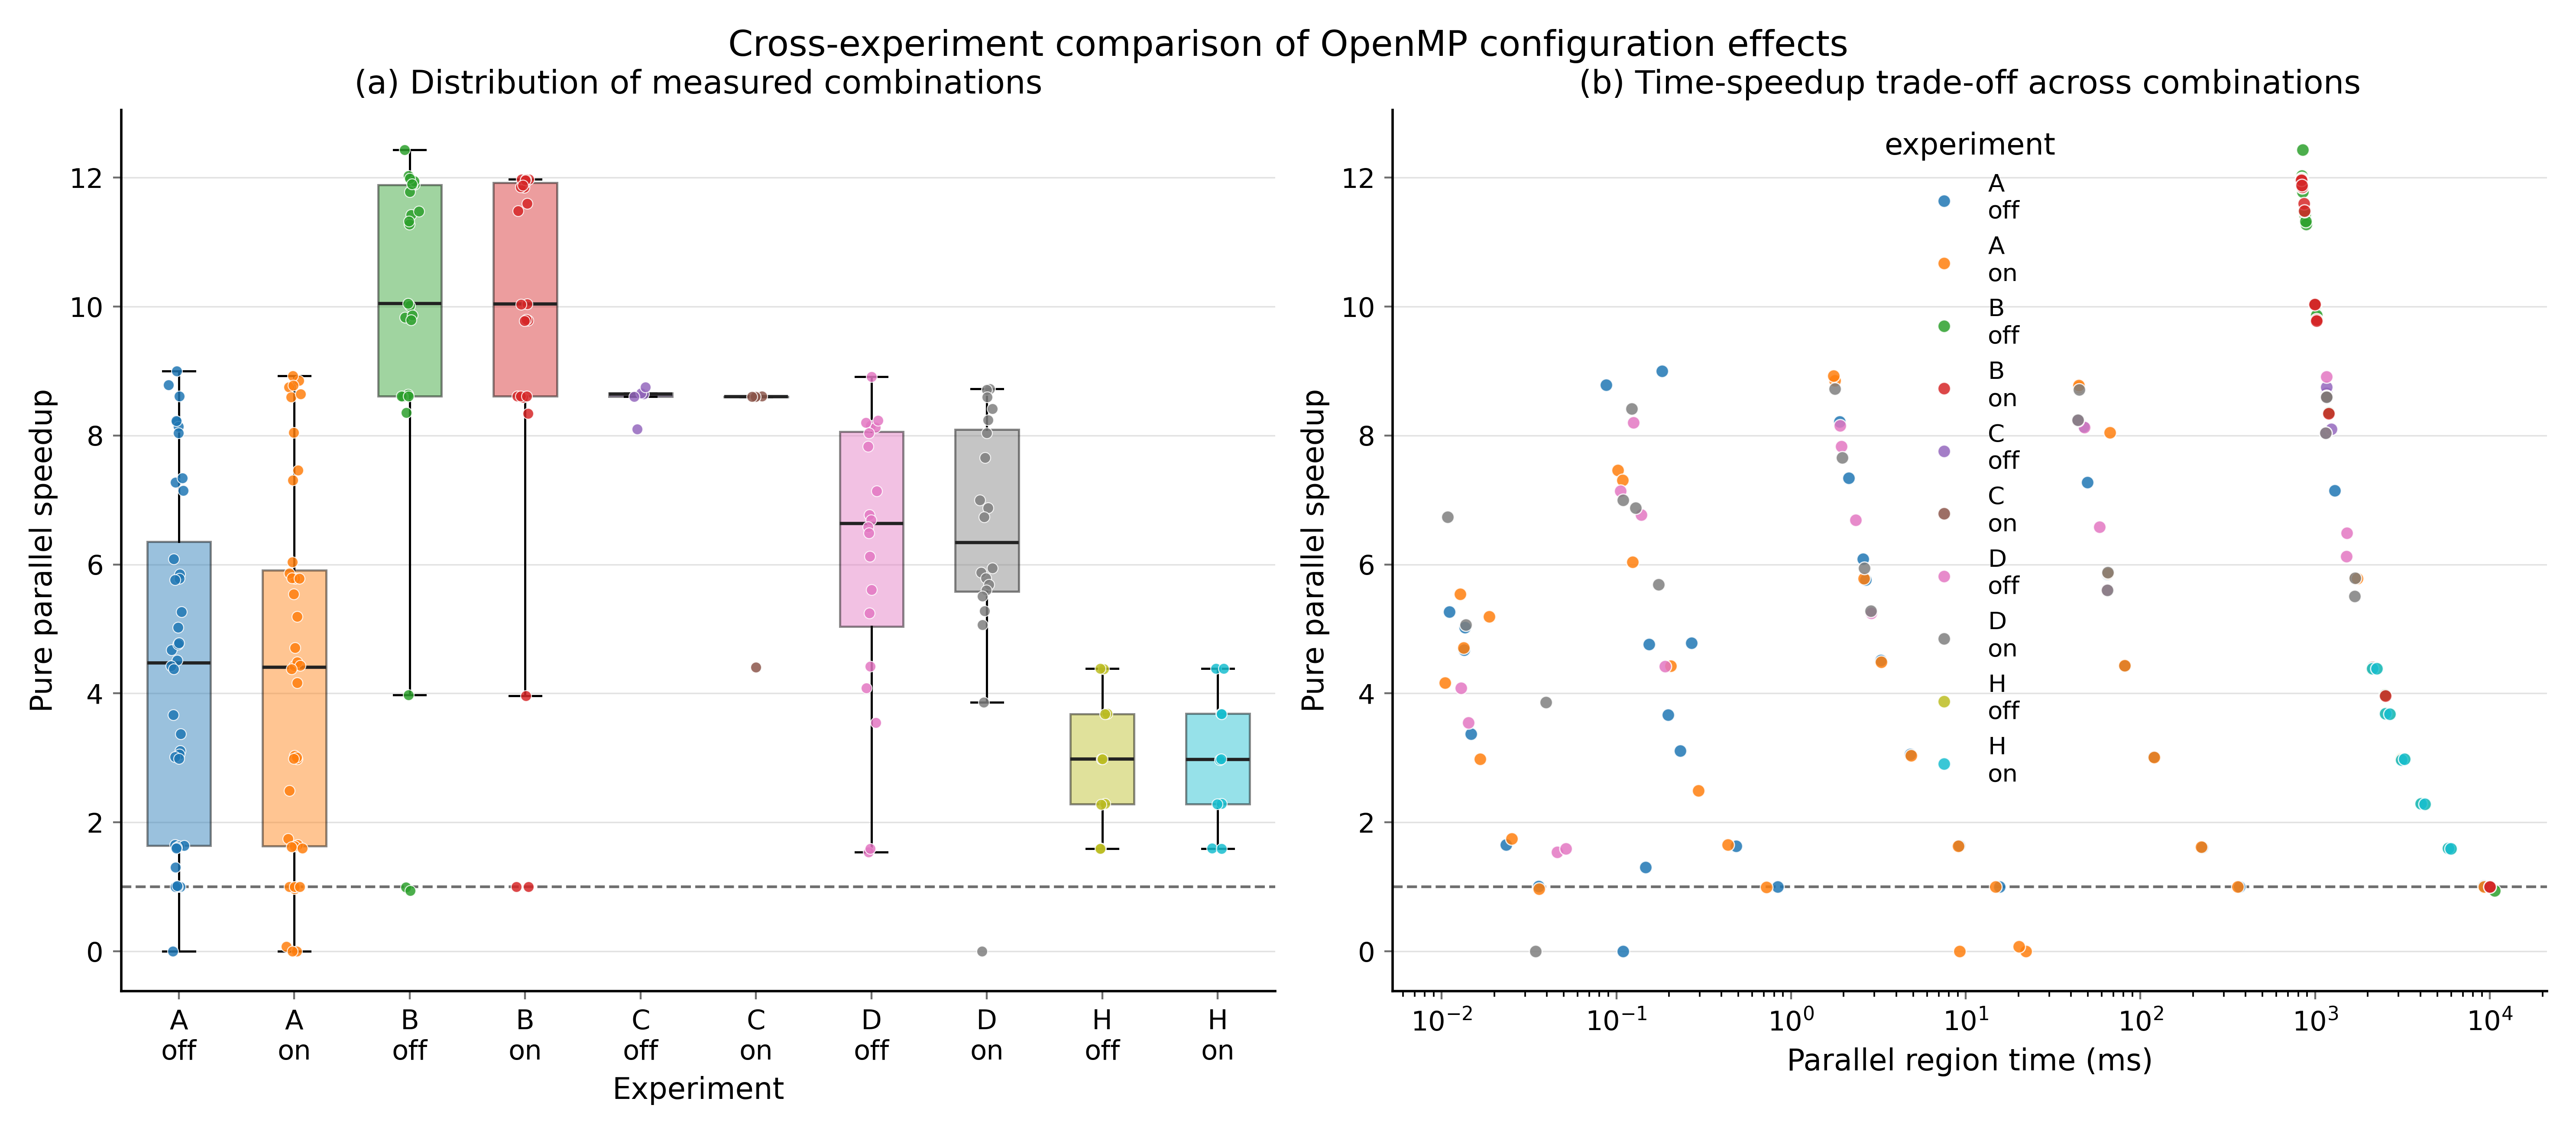
\includegraphics[width=\linewidth]{figure_summary.png}
\caption{OpenMP 설정 및 SMT 조건에 따른 speed up 비교 결과. 
(a)는 각 실험 조건별 pure speedup의 분포이며, (b)는 병렬 영역의 절대 실행 시간에 따른 speedup의 상관관계를 보여주는 scatter plot니다.
두 그래프 모두 스피드업 $1.0$ 지점에 가로 점선으로 기준선을 표시하였다.}
\label{fig:summary}
\end{figure}

\begin{table}[h]
\centering
\small
\textbf{Pure speedup 기준: 높을수록 좋음}\par\medskip
\begin{tabular}{llcc}
\toprule
실험 & 측정값 & SMT-off 최적값 & SMT-on 최적값 \\
\midrule
A Strong scaling & pure speedup & $9.00\times$ & $8.93\times$ \\
B Schedule & pure speedup & $12.43\times$ & $11.98\times$ \\
C 스레드 배치/고정 & pure speedup & $8.75\times$ & $8.61\times$ \\
D Runtime policy & pure speedup & $8.91\times$ & $8.73\times$ \\
H 스레드 배치/고정 compute & pure speedup & $4.38\times$ & $4.38\times$ \\
\bottomrule
\end{tabular}

\vspace{0.8em}
\textbf{Cycle 비용 기준: 낮을수록 좋음}\par\medskip
\begin{tabular}{llcc}
\toprule
실험 & 측정값 & SMT-off 최적값 & SMT-on 최적값 \\
\midrule
E Cache capacity & cycles/load & $3.77$ & $3.78$ \\
F L3/CCD sharing & cycles/load & $5.94$ & $6.14$ \\
G L1/L2 locality & cycles/load & $0.356$ & $0.290$ \\
I 스레드 배치/고정 cache & cycles/load & $0.640$ & $0.769$ \\
J False sharing & cycles/update & $0.124$ & $0.132$ \\
\bottomrule
\end{tabular}
\caption{실험별 최상위 구성 요약. Pure speedup은 fork--join 오버헤드를 제외한 계산 구간 기준.}
\label{tab:result-summary}
\end{table}

\subsection{Experiment A: Strong Scaling}

그림~\ref{fig:exp-a-scaling}은 계산 중심 커널에서 작업 분배 방식과 스레드 배치/고정을 고정하고, 스레드 수와 입력 크기만 변화시킨 결과이다. 단일 스레드 구성의 pure speedup은 SMT-off와 SMT-on 모두 대부분 $1\times$ 부근에 분포하여 기준 실행으로 적절하게 동작하였다. 가장 큰 입력인 $10^7$ 기준 SMT-off에서는 1, 2, 4, 6, 8, 12, 16, 24스레드가 각각 $1.01\times$, $1.60\times$, $2.99\times$, $4.38\times$, $5.78\times$, $8.61\times$, $7.14\times$, $8.04\times$를 기록하였다. 같은 입력에서 SMT-on은 각각 $1.00\times$, $1.60\times$, $2.99\times$, $4.38\times$, $5.79\times$, $8.60\times$, $5.78\times$, $8.64\times$였다.

전체 실험 A의 pure speedup 최대값은 작은 입력에서 관찰되었다. SMT-off에서는 $10^4$ 작업량의 16스레드가 $9.00\times$로 가장 높았고, SMT-on에서는 $10^5$ 작업량의 24스레드가 $8.93\times$로 가장 높았다. 다만 이 구간은 병렬 계산 시간이 ms 이하로 짧아 fork--join 보정과 타이머 잡음의 영향을 크게 받기에 $10^7$를 위주로 해석하는 것이 적절하다고 판단된다. SMT-off의 16 및 24스레드는 물리 코어 수를 넘는 oversubscription 조건이기에 효율은 각각 $0.446$, $0.335$까지 낮아졌다. SMT-on에서도 24스레드 효율은 $0.360$으로, 이 계산 커널에서는 추가 SMT sibling이 12개 물리 코어 대비 큰 이득을 만들지는 못하였다.

\begin{figure}[htbp]
\centering
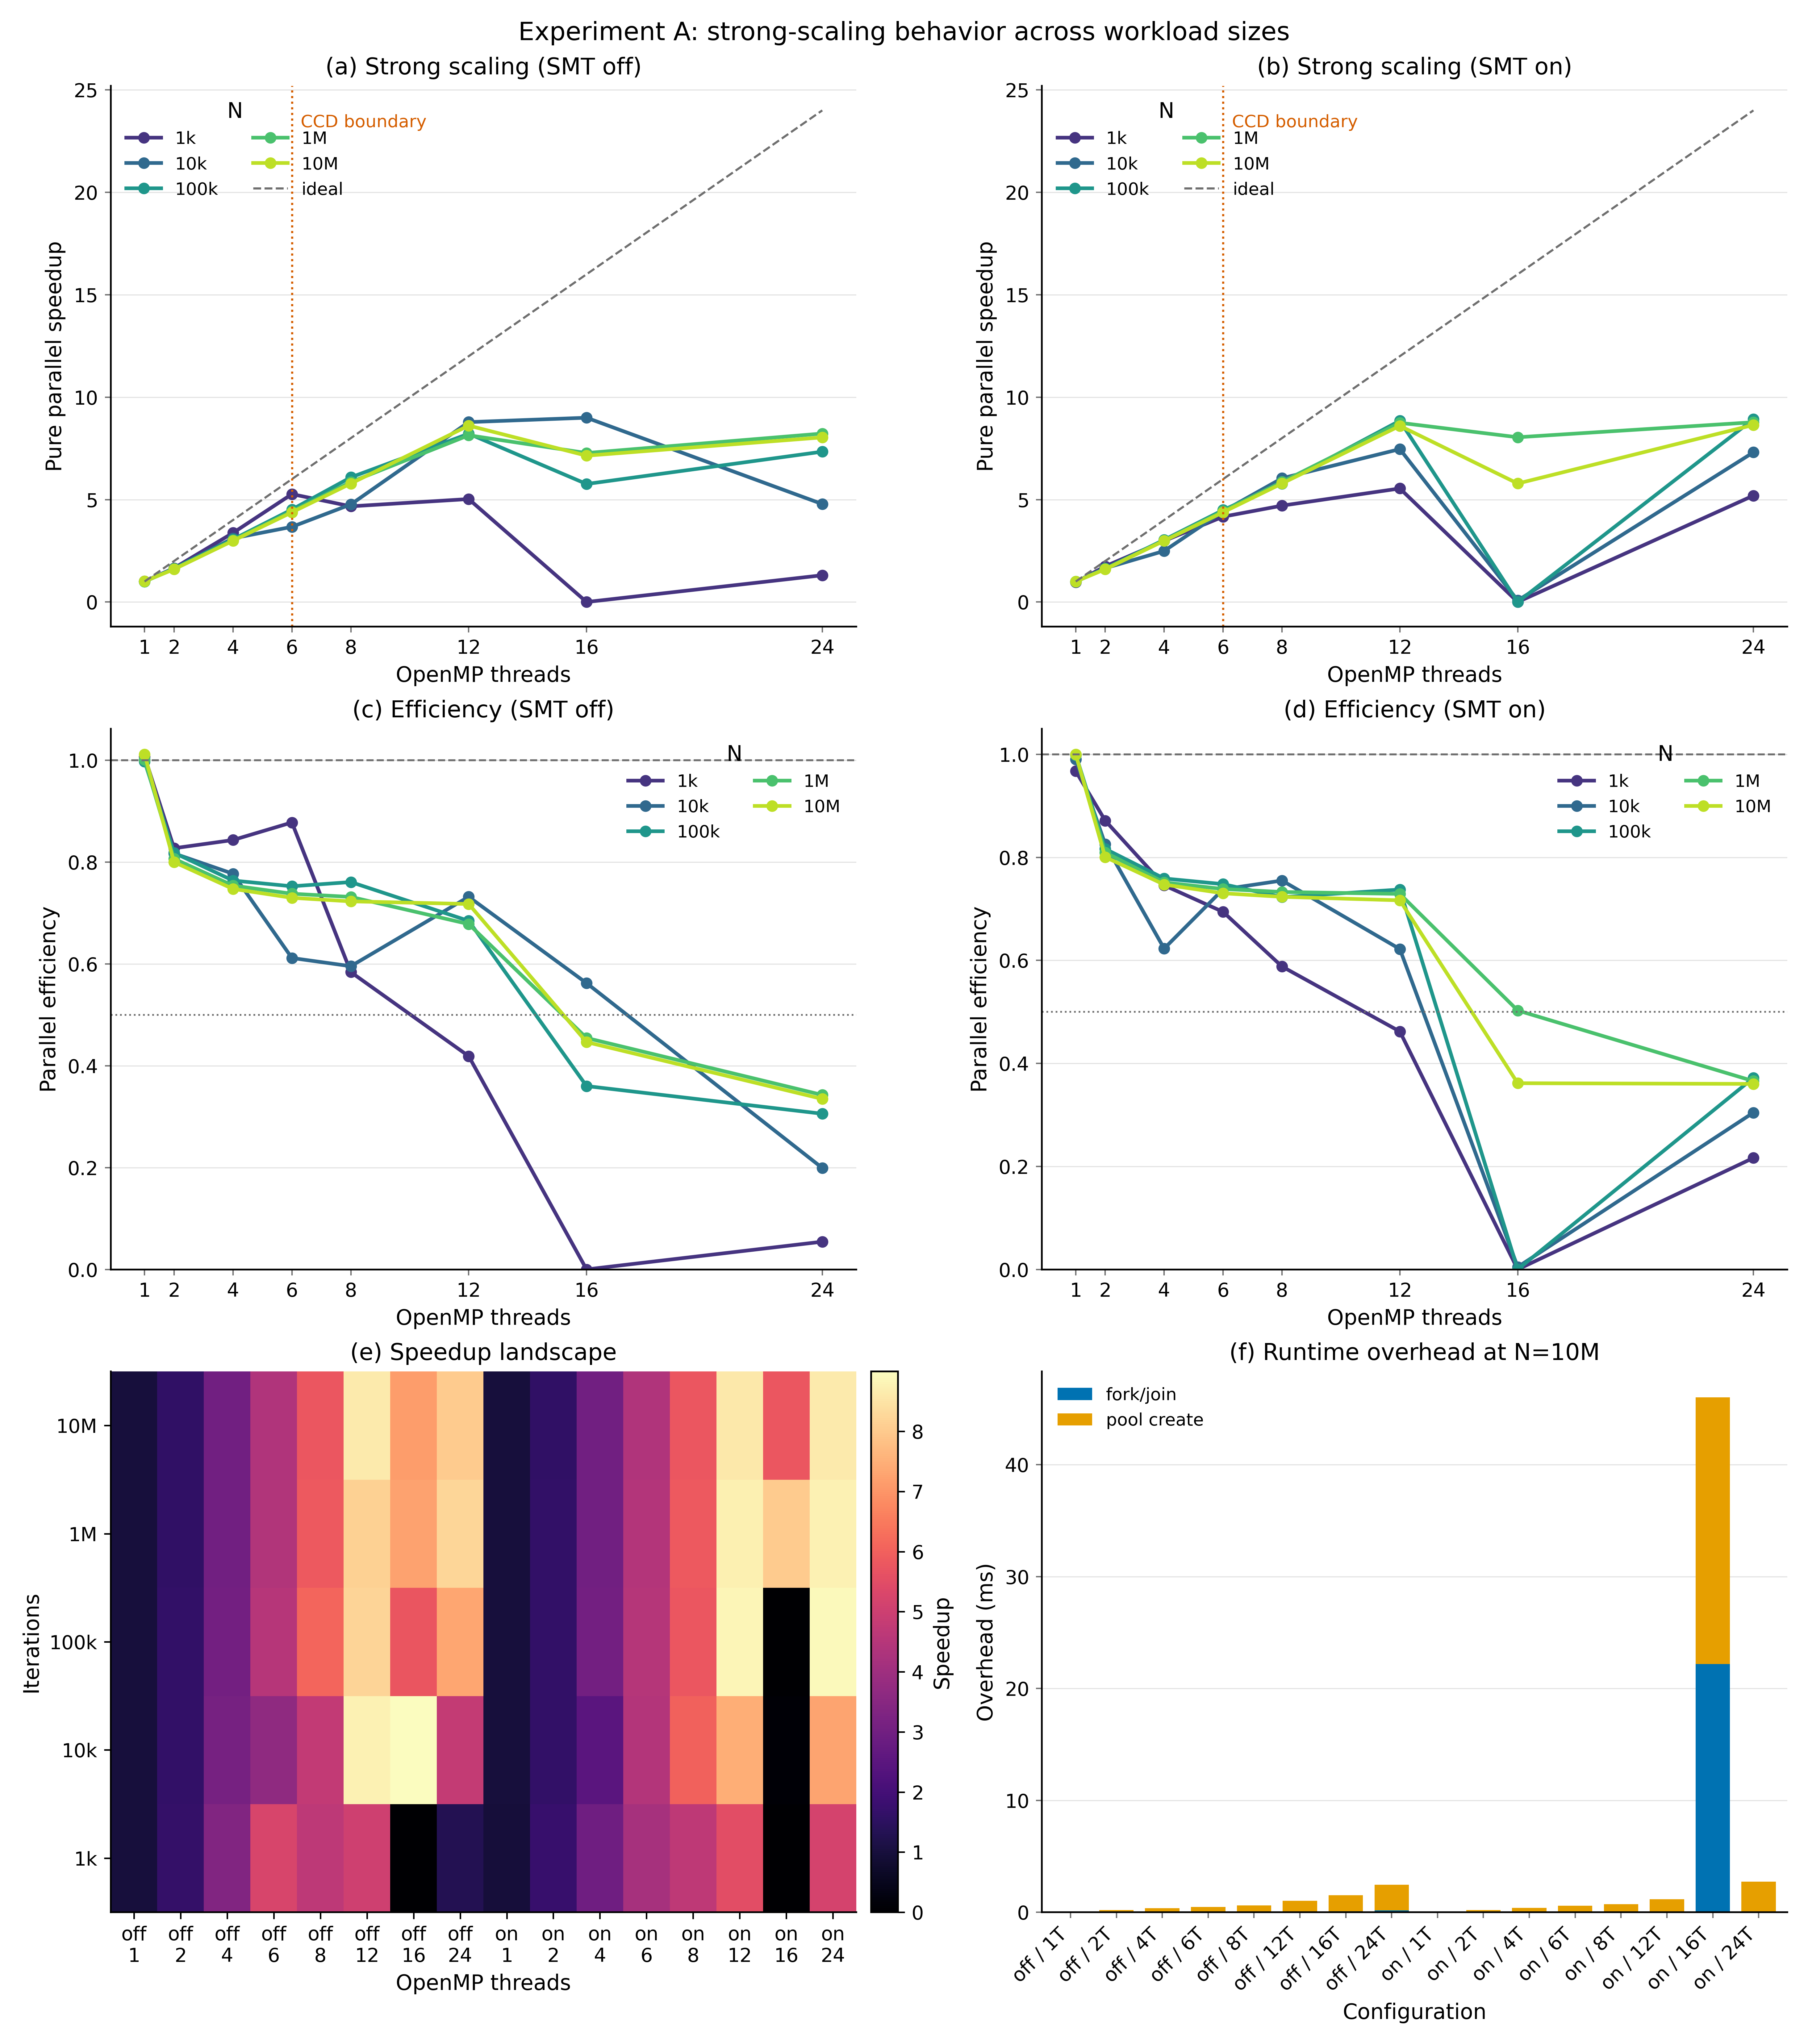
\includegraphics[width=\linewidth]{figure_A_scaling.png}
\caption{실험 A의 확장성, 병렬 효율, pure speedup landscape, 런타임 오버헤드 분석. 병렬 for, static 스케줄, 물리 코어 기준 매핑, 근접 배치 조건으로 수행.
(a, b) SMT 비활성화 및 활성화 환경에서의 pure speedup 비교. $10^7$ 기준, 12스레드는 SMT-off와 SMT-on에서 각각 $8.61\times$, $8.60\times$를 기록했고, 24스레드는 각각 $8.04\times$, $8.64\times$였다.
(c, d) 스레드 수 증가에 따른 병렬 효율 변화. $10^7$ 기준 24스레드 효율은 SMT-off $0.335$, SMT-on $0.360$으로 낮아졌다.
(e) 모든 작업량 및 스레드 구성에 대한 pure speedup 히트맵.
(f) $N=10^7$ 작업량에서의 런타임 오버헤드 분석으로, 많은 스레드 구성에서 계산 시간 대비 fork--join 및 thread pool 관련 오버헤드의 상대적 비중 확인 가능하다.}

\label{fig:exp-a-scaling}
\end{figure}

\subsection{Experiment B: Work Distribution and Scheduling}

그림~\ref{fig:exp-b-schedule}은 12개 물리 코어를 모두 사용하고, 스레드 배치/고정과 런타임 대기 정책을 동일하게 고정한 상태에서 작업 분배 방식과 schedule chunk를 바꾸어 측정한 결과이다.

SMT-off에서 pure speedup은 guided를 큰 chunk로 적용한 구성이 $12.43\times$로 가장 높았다. 같은 guided는 chunk를 기본값으로 두거나 64, 1, 1024로 둔 경우에도 각각 $12.03\times$, $11.99\times$, $11.95\times$, $11.90\times$를 기록해 상위권에 위치하였다. \texttt{tasks} 기반 dynamic 역시 chunk 64 및 1024에서 각각 $11.89\times$로 유사한 성능을 보였다. 반면 단순 연속 static은 $8.63\times$에 머물렀다.

SMT-on에서도 guided와 적절한 chunk를 둔 dynamic이 가장 좋은 결과를 보였다. 최댓값은 guided에서 가장 작은 chunk를 사용한 경우의 $11.98\times$였고, guided의 64 chunk, dynamic의 1024 chunk, guided의 기본 chunk도 모두 $11.97$--$11.98\times$ 범위였다. static도 chunk를 1024로 세분화하면 $11.93\times$로 상위권에 포함되었지만, 단순 연속 static은 $8.59\times$였다. auto schedule는 SMT-off와 SMT-on에서 각각 $8.61\times$, $8.59\times$였다.

하위권에서는 지나치게 작은 static chunk와 작은 task chunk가 낮은 pure speedup을 기록하였다. chunk를 1로 설정한 static은 SMT-off와 SMT-on에서 각각 $3.97\times$, $3.96\times$였고, \texttt{tasks} 기반 작업 분배 방식도 chunk가 256 또는 8192로 작을 때는 두 SMT 조건에서 약 $0.94$--$1.00\times$ 수준에 머물렀다. 반면 \texttt{tasks}도 chunk를 충분히 키우니 약 $8.3\times$까지 회복되었다.

\begin{figure}[h]
\centering
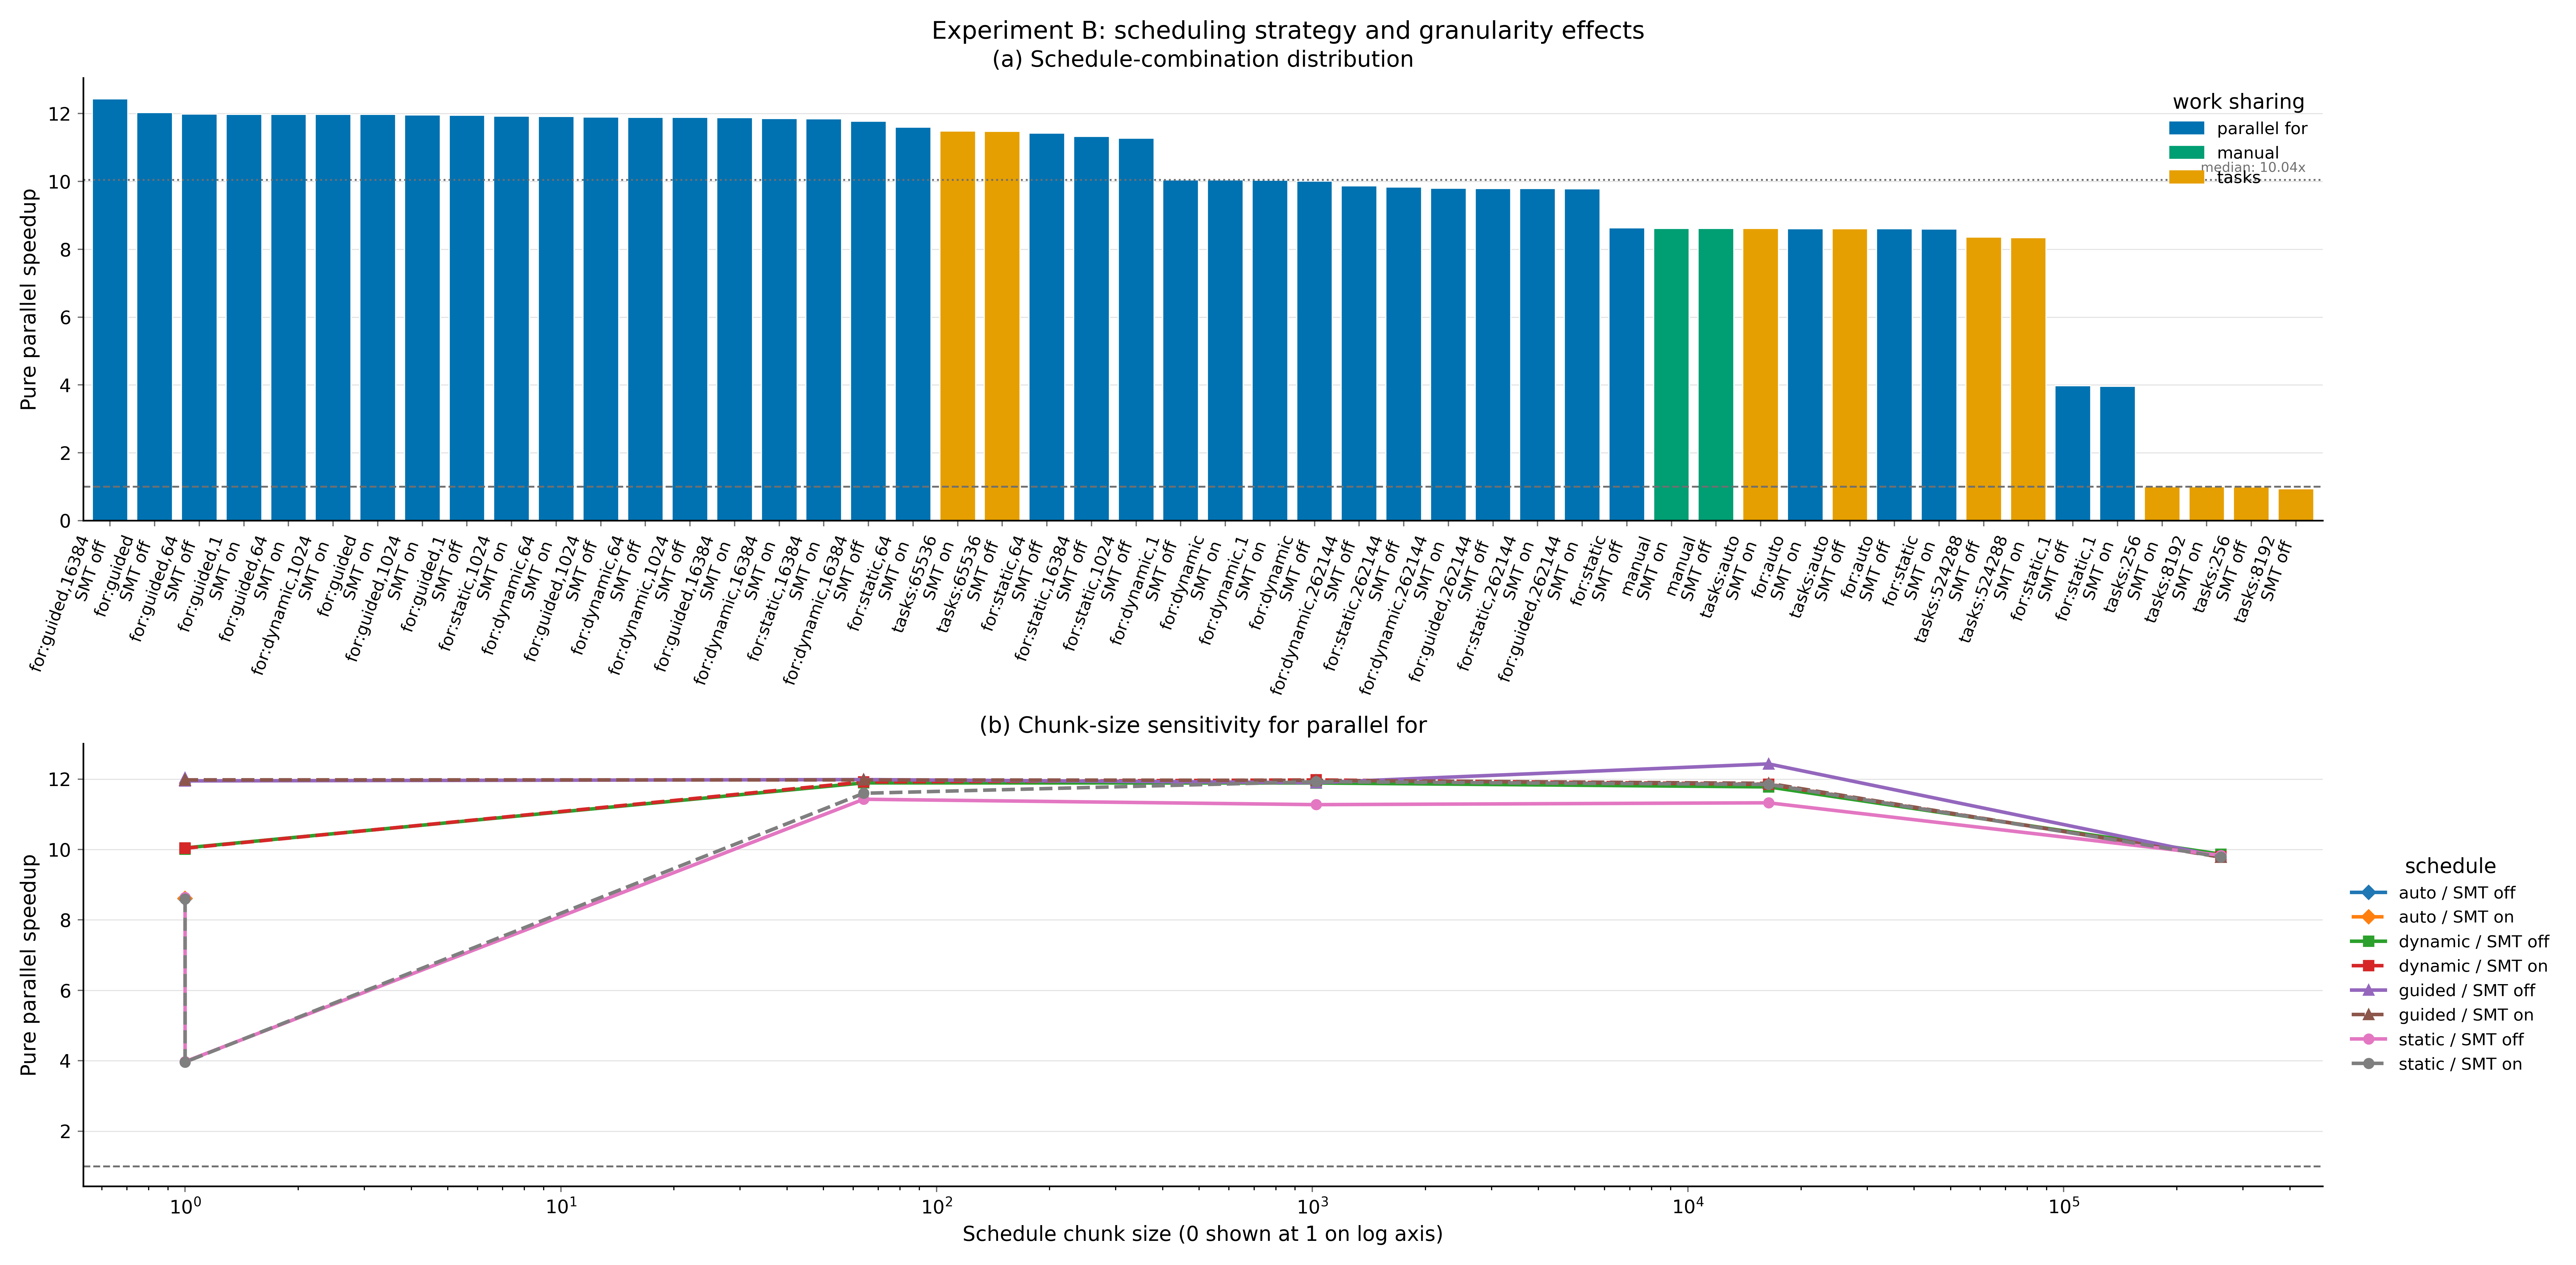
\includegraphics[width=\linewidth]{figure_B_schedule.png}
\caption{실험 B의 작업 분배 방식 및 스케줄링 결과. (a) 12스레드 조건에서 작업 분배 방식과 schedule 조합별 pure speedup. 파란색이 \texttt{parallel\_for}, 초록색이 \texttt{manual}, 주황색이 \texttt{tasks}이다. (b) \texttt{parallel\_for}에 대해 schedule 종류와 chunk 크기에 따른 pure speedup 변화를 SMT-off 및 SMT-on 조건별로 비교한다. 입력 크기와 스레드 수는 고정하였으며, guided와 적절한 chunk를 둔 dynamic은 상위권에 분포하고 단순 연속 static 및 지나치게 작은 static chunk는 상대적으로 낮게 나타난다.}
\label{fig:exp-b-schedule}
\end{figure}

\subsection{Experiment C: Thread Placement and Pinning}

그림~\ref{fig:exp-c-affinity}는 동일한 계산 커널에서 스레드 배치/고정 방식만 바꾸어 측정한 실험 C의 결과이다. 입력 크기는 $10^7$로 고정하고 12개 스레드가 병렬 for와 static 스케줄로 수행하도록 하였다. 모든 실행에서 런타임이 실제로 사용한 스레드 수 역시 12개였다.

SMT-off에서는 물리 코어 단위로 넓게 분산 배치한 경우가 pure speedup $8.75\times$로 가장 높았고, 해당 구성의 병렬 실행 시간은 1159.34\,ms였다. 물리 코어 단위의 근접 배치, 논리 스레드 단위의 근접 배치, 논리 스레드 단위의 분산 배치는 각각 $8.66\times$, $8.65\times$, $8.61\times$로 서로 큰 차이가 없었다. 반면 스레드 고정을 사용하지 않은 경우는 $8.10\times$, 1237.92\,ms로 가장 낮았다.

SMT-on에서는 스레드 고정을 사용하지 않은 경우와 물리 코어 단위의 분산 배치가 모두 $8.61\times$로 가장 높은 범위에 있었고, 병렬 실행 시간은 약 1161\,ms였다. 논리 스레드 단위의 분산 배치와 물리 코어 단위의 근접 배치 역시 $8.59$--$8.60\times$로 큰 차이가 없었다. 반면 논리 스레드 단위의 근접 배치는 $4.41\times$, 2125.41\,ms로, SMT-on의 다른 배치 조합보다 뚜렷하게 낮은 pure speedup과 긴 병렬 실행 시간을 보였다.

\begin{figure}[h]
\centering
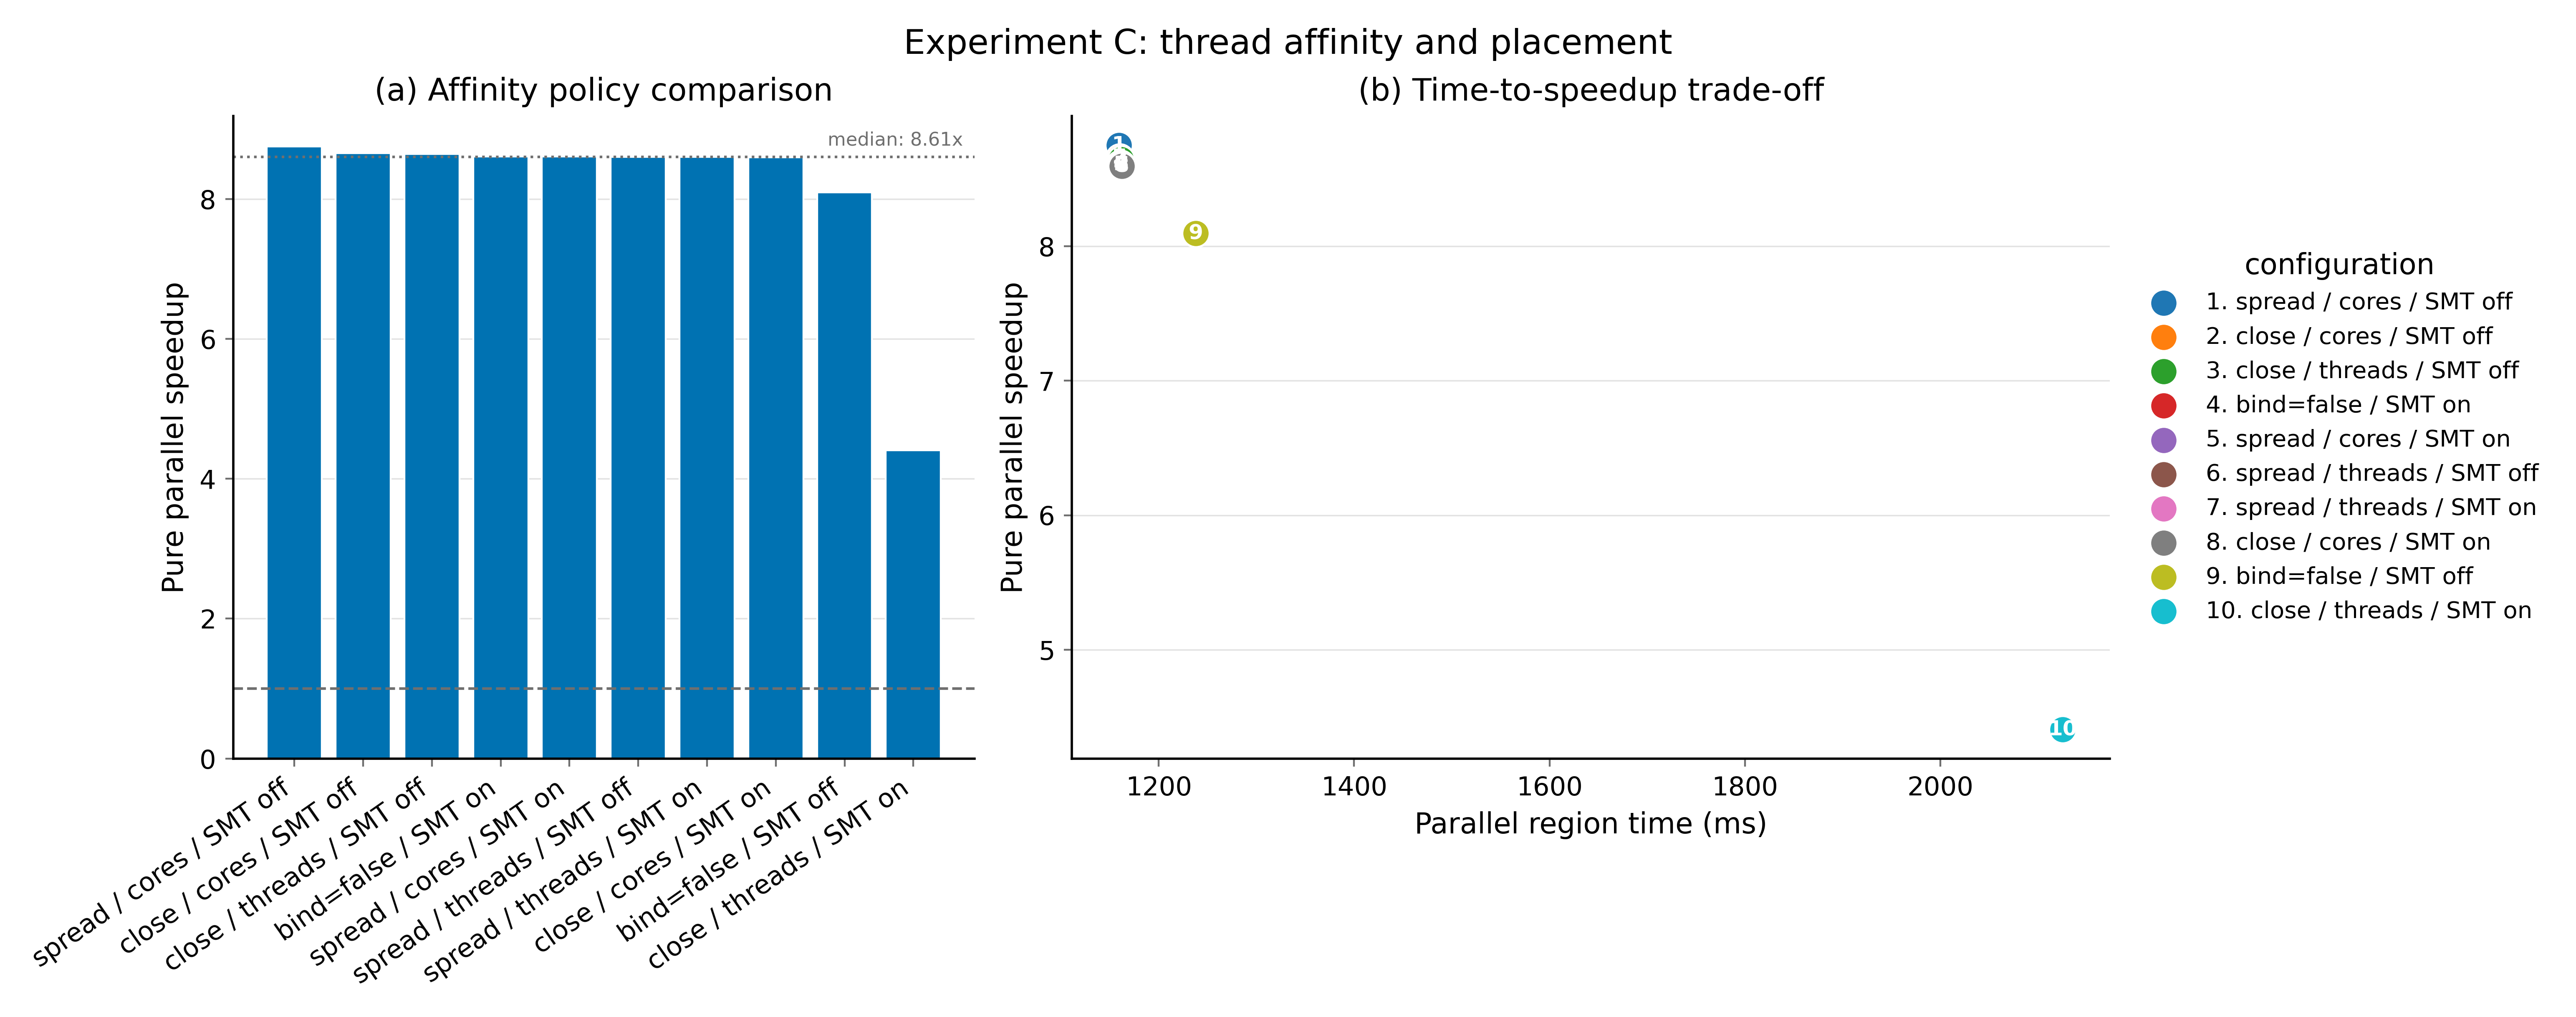
\includegraphics[width=\linewidth]{figure_C_affinity.png}
\caption{실험 C의 스레드 배치/고정 결과. (a) 각 배치 조합의 pure speedup, (b) 동일한 조합을 병렬 실행 시간과 pure speedup의 관계. 입력 크기와 스레드 수는 고정, 스레드 고정 미사용, 근접 배치, 분산 배치를 물리 코어 단위와 논리 스레드 단위로 비교하였다. 대부분의 조합은 $8.6\times$ 안팎에 모여 있지만, SMT-on의 논리 스레드 단위 근접 배치는 실행 시간이 길고 pure speedup이 낮게 나타난다.}
\label{fig:exp-c-affinity}
\end{figure}

\subsection{Experiment D: Runtime Policy}

그림~\ref{fig:exp-d-runtime}은 계산 커널, 병렬 for, static 스케줄, 스레드 12개, 물리 코어 기준 근접 배치로 고정하고 스레드 대기 정책과 dynamic 스레드 수 조절 여부만 바꾸어 측정한 결과이다. dynamic 스레드 조절을 끈 경우에는 모든 실행에서 실제 스레드 수가 12개로 유지되었다. 반면 dynamic 조정을 켠 경우에는 런타임이 스레드 수를 줄인 것을 확인하였다. SMT-off에서는 active policy가 스레드 9개를 사용하였고, passive policy는 스레드 8개, $10^7$에선 스레드 9개를 사용하였다. SMT-on에서는 두 policy 모두 스레드 8개로 실행됨을 확인하였다.

SMT-off에서 가장 높은 pure speedup은 active에 고정 스레드 수를 사용하였을 때, $10^7$에서 $8.91\times$였다. passive에 고정 스레드 수를 사용한 경우에는 $8.04\times$였고, dynamic에서는 실제 스레드 수가 줄어든 영향으로 active $6.49\times$, passive $6.12\times$에 머물렀다.

SMT-on에서도 active 대기와 고정 스레드 수를 사용한 구성이 가장 높은 pure speedup을 기록하였다. 비교적 작은 입력인 $10^5$에서는 $8.73\times$을 보였으며, $10^7$에서는 $8.59\times$를 보였다. passive에 고정 스레드 수를 사용한 경우는 $10^7$에서 $8.04\times$를 기록하였다. dynamic에서는 실제 스레드 수가 8개로 줄었고, $10^7$ active는 $5.79\times$, passive는 $5.51\times$였다.

전체 실행 시간은 크기 축 기준으로 단조 증가 함수 꼴이었다. $10^7$ 기준 SMT-off의 실행 시간은 active/고정 스레드 $9.50$\,s, passive/고정 스레드 $8.42$\,s, active/동적 조정 $9.22$\,s, passive/동적 조정 $8.72$\,s였다. SMT-on에서는 같은 순서로 $9.05$\,s, $8.43$\,s, $9.32$\,s, $8.86$\,s가 기록되었다. 병렬 영역 진입 및 종료 오버헤드는 $10^7$ 기준 active에서 약 $0.006$--$0.008$\,ms, passive에서 약 $0.026$--$0.034$\,ms 범위였다.

\begin{figure}[h] 
\centering
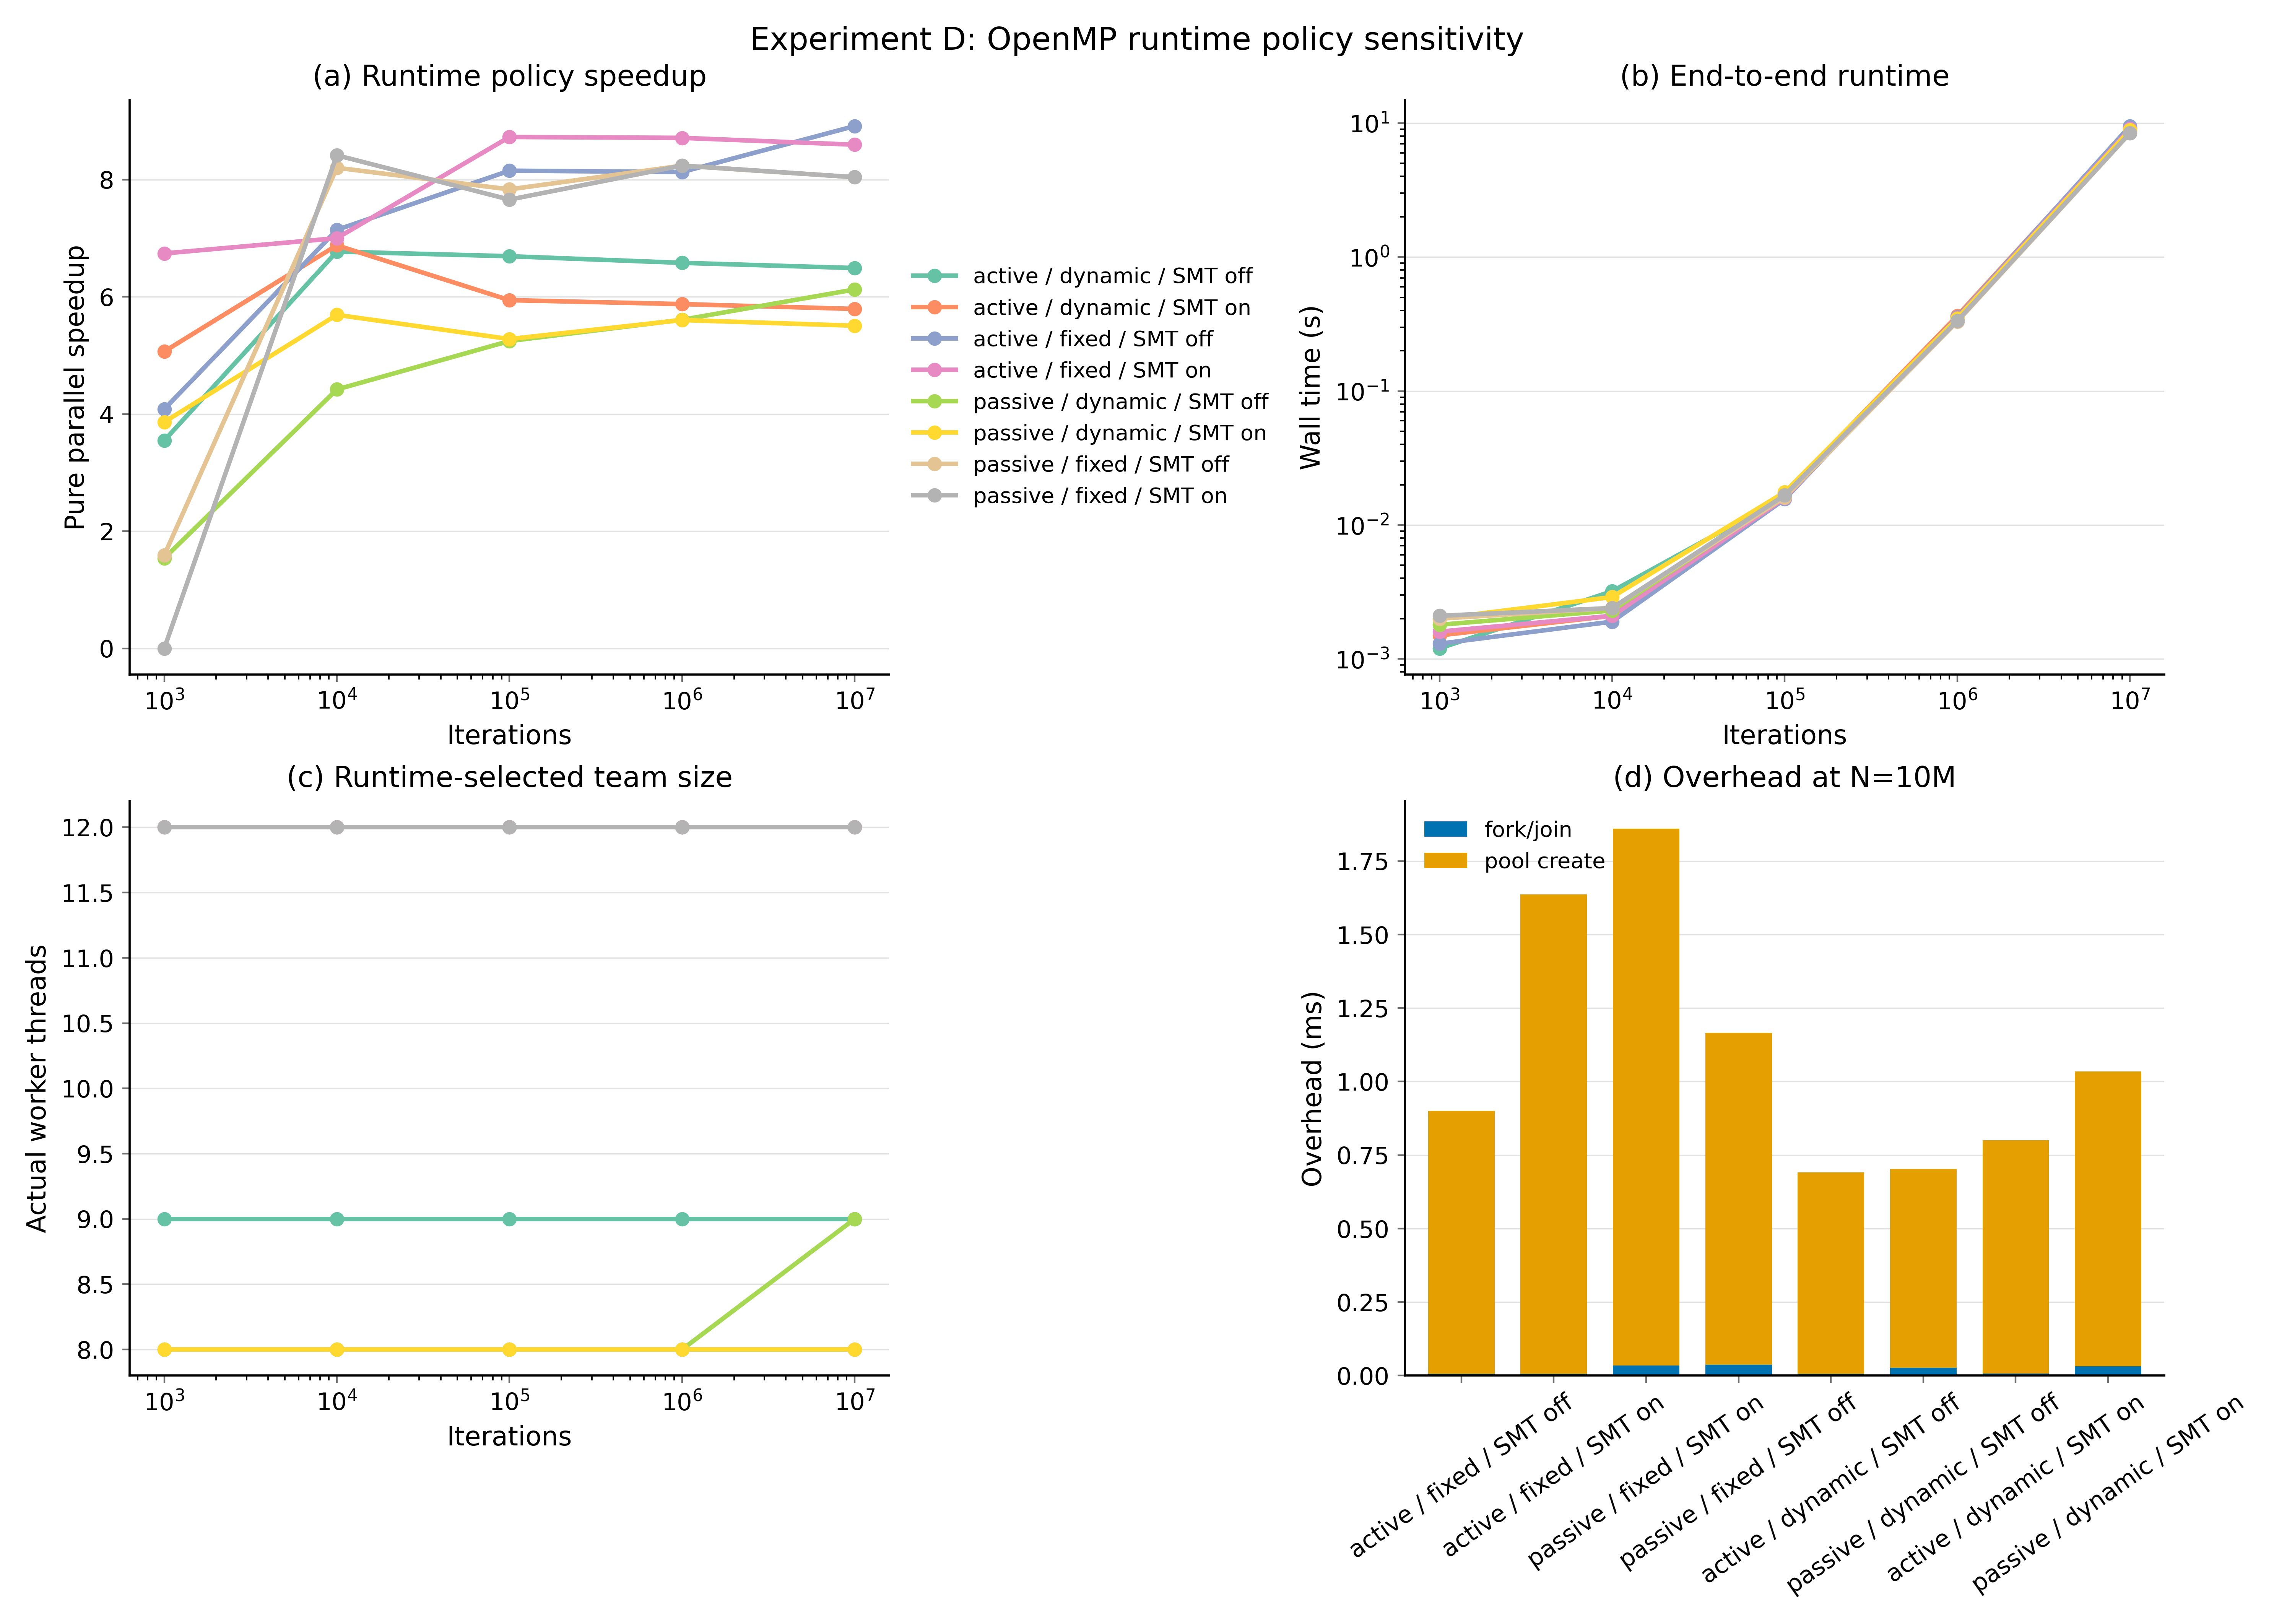
\includegraphics[width=\linewidth]{figure_D_runtime.png}
\caption{실험 D의 OpenMP 런타임 정책에 따른 성능 민감도 분석 결과. 모든 실험은 12개의 스레드를 물리 코어에 근접 배치한 상태에서 측정되었다. (a)는 반복 횟수 증가에 따른 pure speedup 변화를 나타내며, 대기 정책, 스레드 수 조절, SMT 조합에 따른 결과를 비교한다. (b)는 동일한 x축에 대한 전체 실행 시간을 나타내는 그래프로, 입력 크기에 따른 단조 증가 양상을 보여준다. (c)는 런타임에 의해 실제 할당된 스레드 수를 보여주는 그래프로, fixed 설정 시 12개로 고정되는 선형과 dynamic 설정 시 8--9개로 스레드 수가 감소를 확인할 수 있다. (d)는 반복 횟수 $10^7$ 기준 각 설정별 발생 오버헤드를 나타내는 누적 막대 그래프로, 스레드 풀 생성과 fork--join에 소요되는 시간을 분리하여 나타낸다.}
\label{fig:exp-d-runtime}
\end{figure}

\subsection{Experiment E: Cache Capacity Breakpoints}

그림~\ref{fig:exp-e-cache}는 단일 스레드 pointer chase 커널, active 대기, dynamic 스레드 조절 off, CPU 집합 auto 조건으로 working set 크기를 바꾸어 측정한 실험 E의 결과이다. SMT-off와 SMT-on 모두 원소 수 512부터 16\,777\,216까지가 사용되었다. 이때, 모든 실행에서 실제 OpenMP 스레드 수는 1로 기록되었다. 그림의 working set 범위는 4\,KiB부터 128\,MiB까지이다.

SMT-off의 dependent load당 cycle은 4--32\,KiB 구간에서
$3.77$--$3.78$ cycles/load로 측정되었다. 64\,KiB에서는
$7.05$ cycles/load였고, 128\,KiB와 256\,KiB에서는 각각
$8.50$, $10.07$ cycles/load였다. 512\,KiB에서는 $16.12$ cycles/load,
1\,MiB에서는 $27.75$ cycles/load가 기록되었다. 2--8\,MiB 구간은
$34.42$--$35.14$ cycles/load 범위였으며, 16\,MiB와 32\,MiB에서는
각각 $35.32$, $48.03$ cycles/load였다. 64\,MiB와 128\,MiB에서는
각각 $209.01$, $280.28$ cycles/load로 측정되었다.

SMT-on의 dependent load당 cycle도 같은 working set 순서로 기록되었다.
4--32\,KiB 구간은 $3.78$--$3.84$ cycles/load였고, 64\,KiB에서는
$7.09$ cycles/load였다. 128\,KiB와 256\,KiB는 각각 $8.50$,
$10.12$ cycles/load였으며, 512\,KiB와 1\,MiB에서는 각각 $17.38$,
$28.58$ cycles/load였다. 2--8\,MiB 구간은 $35.32$--$36.22$
cycles/load 범위에 있었고, 16\,MiB와 32\,MiB에서는 각각 $36.38$,
$51.61$ cycles/load였다. 64\,MiB와 128\,MiB에서는 각각 $214.08$,
$283.53$ cycles/load로 측정되었다.

절대 실행 시간인 serial timed region은 working set 증가에 따라 함께
증가하였다. SMT-off에서는 32\,KiB $15.86$\,ms, 512\,KiB
$67.62$\,ms, 32\,MiB $805.75$\,ms, 128\,MiB $18.81$\,s가 기록되었다.
SMT-on에서는 같은 working set에서 각각 $16.12$\,ms, $72.90$\,ms,
$865.86$\,ms, $19.03$\,s가 기록되었다.

\begin{figure}[h]
\centering
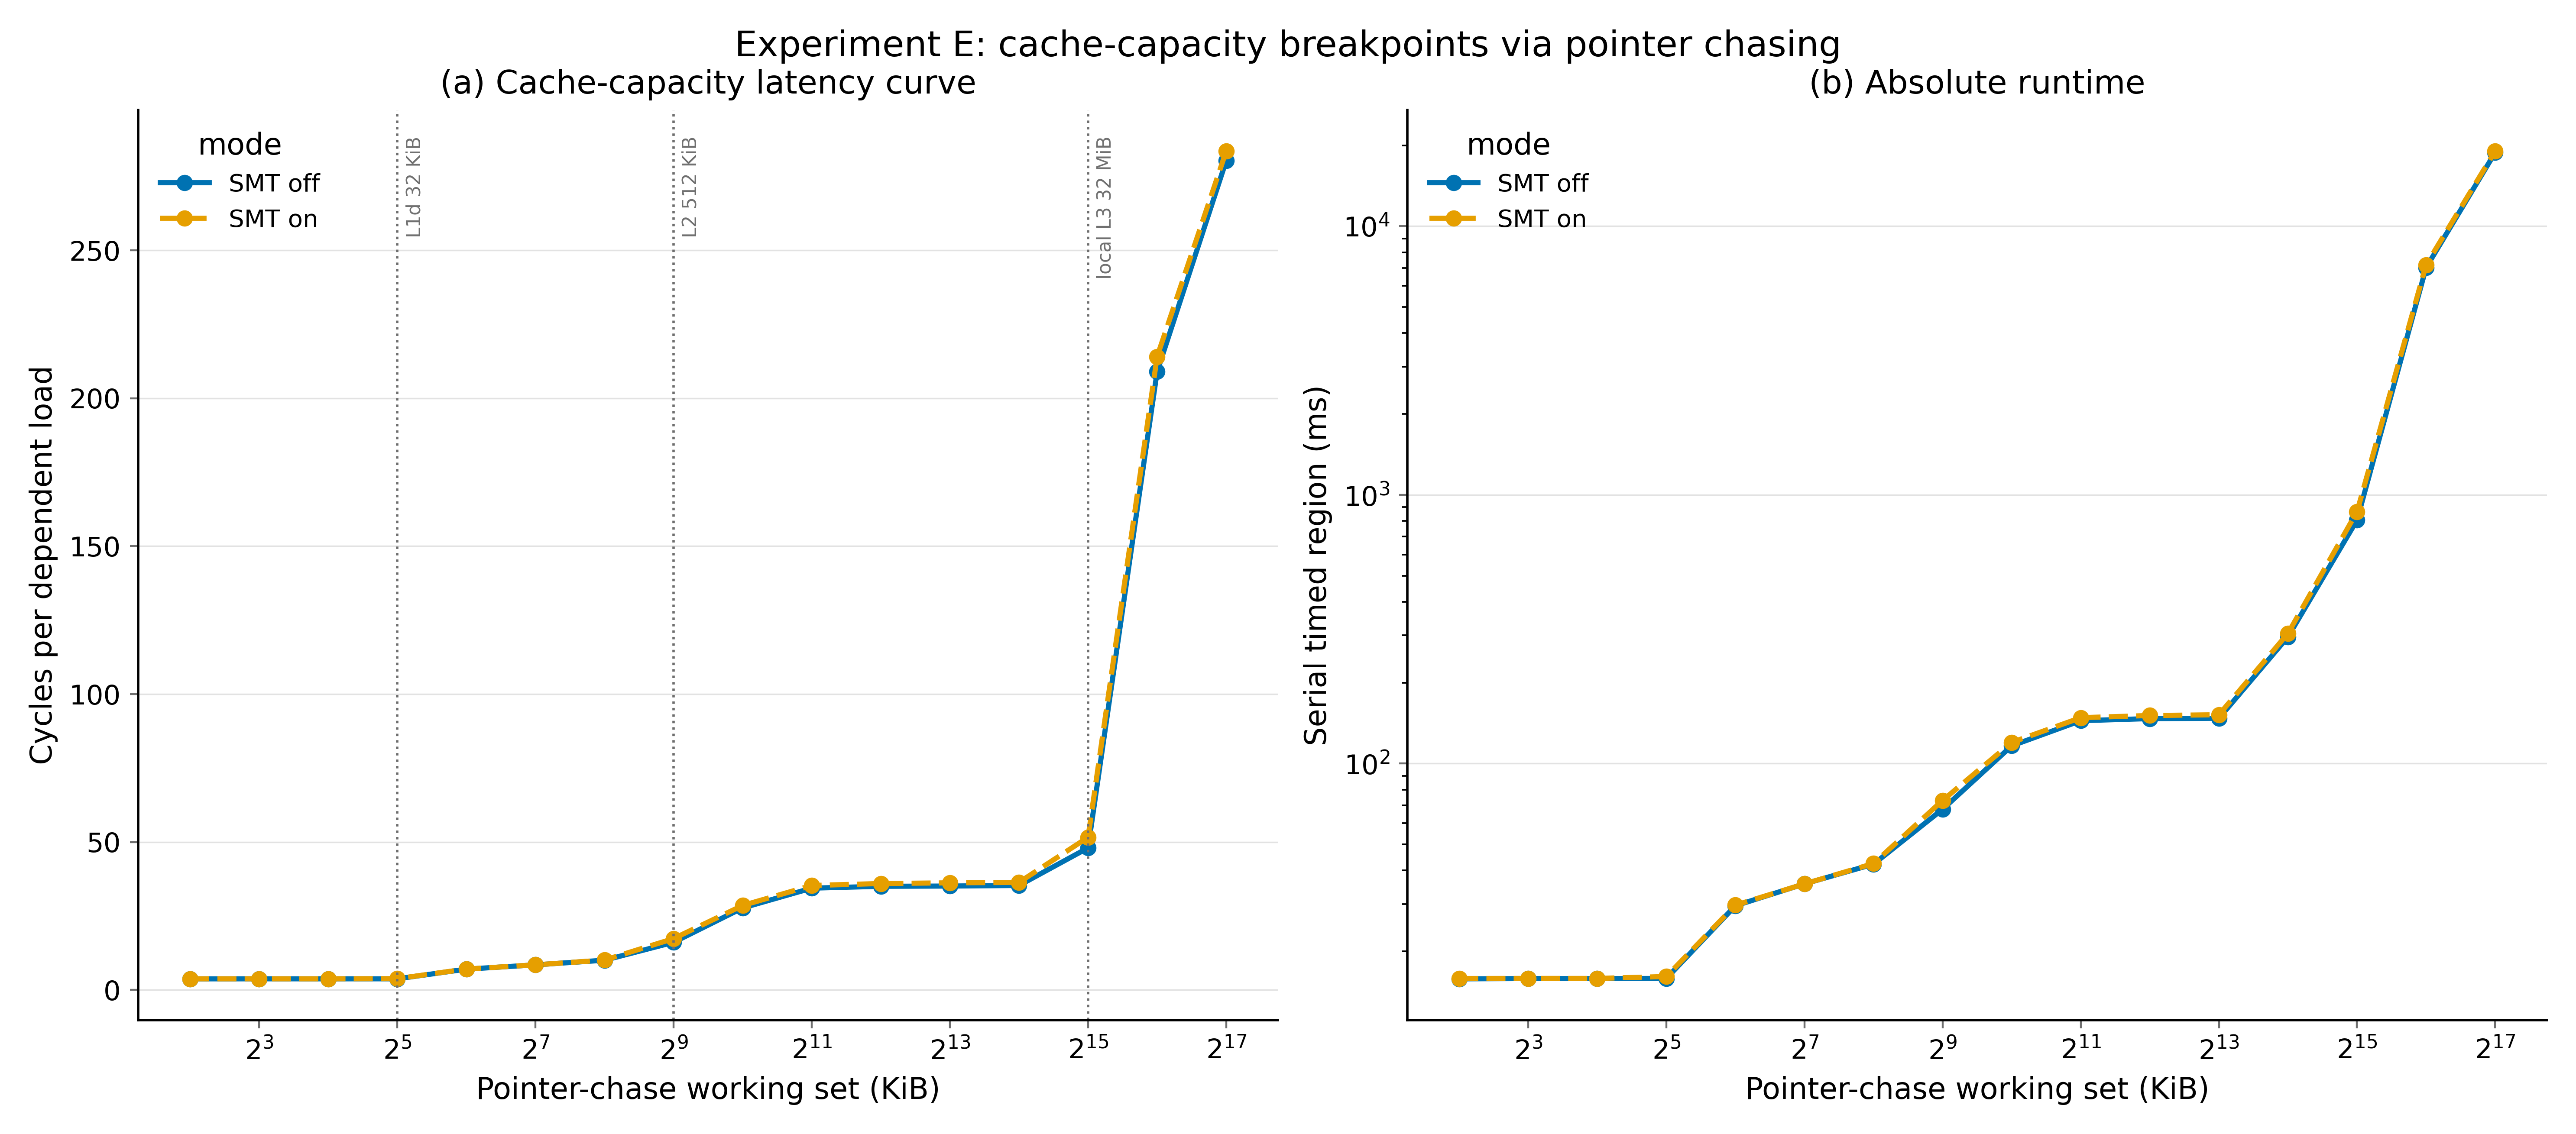
\includegraphics[width=\linewidth]{figure_E_cache.png}
\caption{실험 E의 단일 스레드 pointer chase 커널을 이용한 cache capacity breakpoint 측정 결과. 
(a)는 working set 크기 변화에 따른 dependent load당 소요 cycle을 나타낸 지연 시간 곡선이다. L1d, L2, Local L3 캐시의 물리적 한계 지점이 수직 점선으로 표시되어 있다. (b)는 동일한 working set 변화에 대한 전체 구간 실행 시간을 나타내며, y축에 로그 스케일이 적용되었다. 두 그래프 모두 파란색 실선은 SMT-off, 주황색 점선은 SMT-on 환경에서의 측정값을 의미한다. 4\,KiB부터 128\,MiB 구간에서 각 레벨의 캐시 용량 경계를 초과할 때마다 메모리 접근 지연 시간과 전체 실행 시간이 계단식으로 급증하는 양상을 확인할 수 있으며, 두 SMT 모드 간의 유의미한 성능 궤적 차이는 관찰되지 않았다.}
\label{fig:exp-e-cache}
\end{figure}

\subsection{Experiment F: L3 Sharing Across CCDs}

그림~\ref{fig:exp-f-l3-ccd}는 pointer chase 공유 커널, 스레드 6개,
근접 배치, 물리 코어 기준 매핑, 활성 대기, 동적 스레드 조절 끔을 고정하고, 같은 공유 pointer chase working set을 단일 CCD 배치(0--5)와 둘로 나눈 CCD 배치(0--2, 6--8) 에서 측정한 결과이다. 모든 실행에서 실제 OpenMP 스레드 수는 6으로 확인되었다.

SMT-off에서는 4--16\,MiB 구간의 dependent load당 cycle이 단일 CCD 배치에서 $6.35$, $6.39$, $5.94$ cycles/load였고, CCD 분할 배치에서 $6.15$, $6.20$, $6.25$ cycles/load였다. 32\,MiB에서는 단일 CCD 배치가 $7.54$ cycles/load, CCD 분할 배치가 $7.99$ cycles/load로 측정되었다. 64\,MiB에서는 각각 $34.81$, $34.94$ cycles/load였고, 128\,MiB에서는 각각 $48.54$, $49.19$ cycles/load가 기록되었다.

SMT-on에서는 4--16\,MiB 구간에서 단일 CCD 배치가 $6.14$, $6.31$, $6.19$ cycles/load였고, CCD 분할 배치는 $6.64$, $6.54$, $6.45$ cycles/load였다. 32\,MiB에서는 단일 CCD 배치가 $8.12$ cycles/load, CCD 분할 배치가 $8.77$ cycles/load였다. 64\,MiB에서는 각각 $35.49$, $35.43$ cycles/load, 128\,MiB에서는 각각 $48.93$, $49.54$ cycles/load로 측정되었다.

pure speedup 기준으로는 SMT-off의 CCD 분할 배치가 4--32\,MiB 구간에서 $5.92$, $5.95$, $5.95$, $6.23\times$를 기록하였고, 단일 CCD 배치는 같은 구간에서 $5.49$, $5.49$, $5.94$, $6.02\times$였다. 64\,MiB와 128\,MiB에서는 단일 CCD 배치가 각각 $5.82$, $5.70\times$, CCD 분할 배치가 각각 $5.97$, $5.67\times$로 기록되었다. SMT-on에서는 32\,MiB에서 단일 CCD 배치가 $6.24\times$, CCD 분할 배치가 $6.12\times$였고, 64\,MiB와 128\,MiB에서는 각각 $5.85$ 대 $5.97\times$, $5.72$ 대 $5.72\times$로 측정되었다.

\begin{figure}[h]
\centering
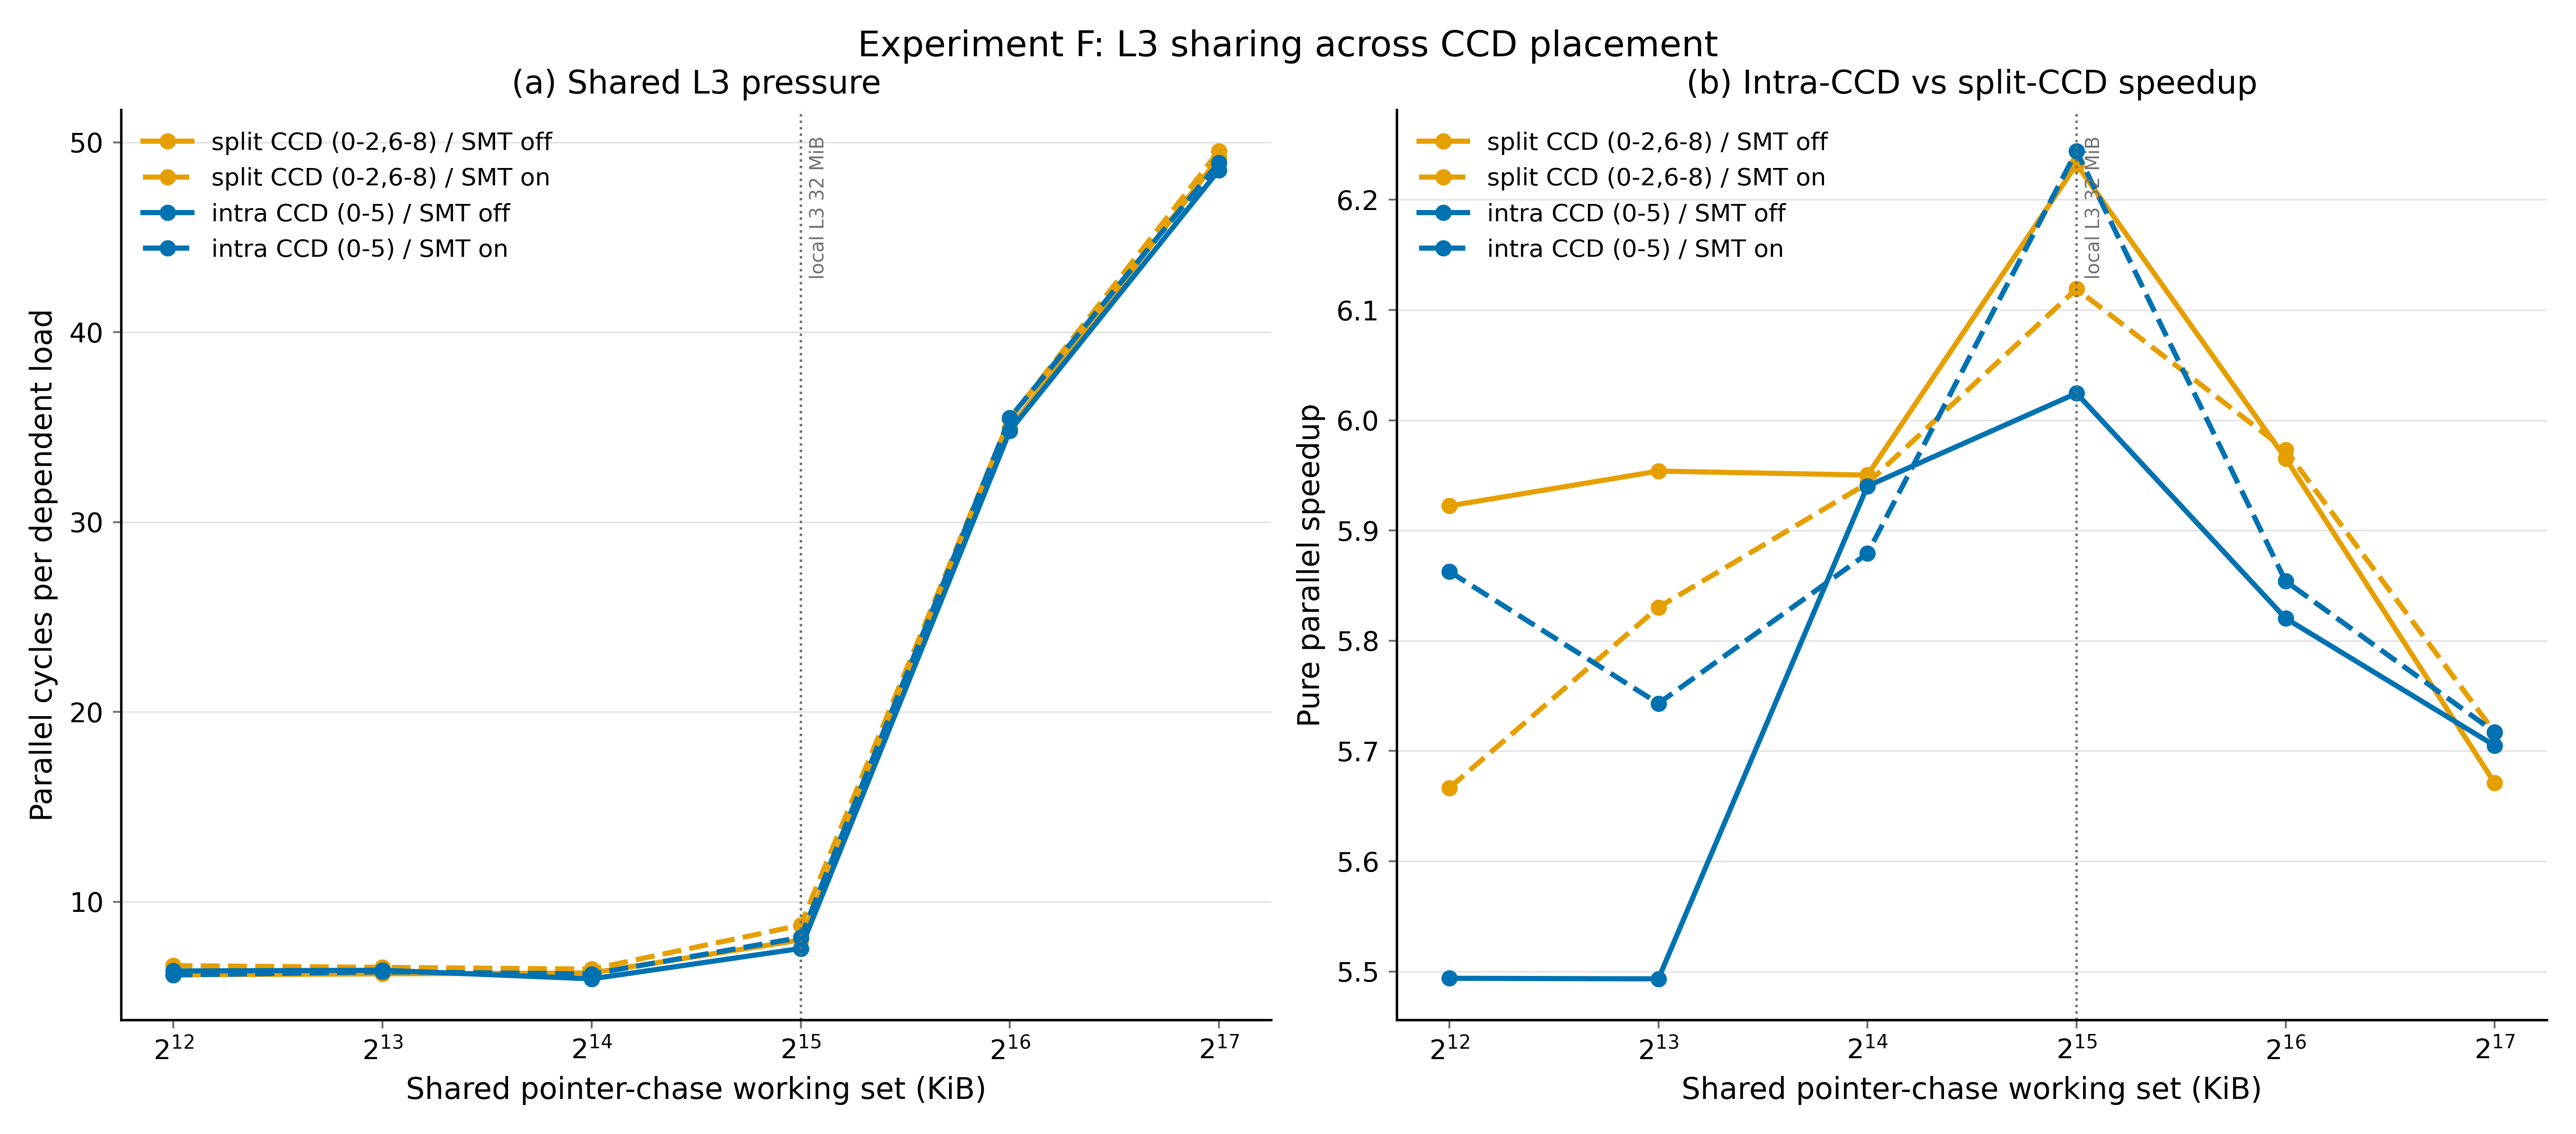
\includegraphics[width=\linewidth]{figure_F_l3_ccd.png}
\caption{실험 F의 6스레드 공유 working set pointer chase 커널을 이용한 L3 캐시 공유 및 스레드 배치에 따른 성능 측정 결과. (a)는 working set 크기 변화에 따른 병렬 dependent load당 소요 cycle을 나타낸 그래프이다. (b)는 동일한 working set 변화에 대한 pure speedup 양상을 보여준다. 두 그래프 모두 파란색 선은 스레드를 단일 CCD(0--5)에 집중 배치한 조건을, 주황색 선은 두 개의 CCD(0--2, 6--8)에 분산 배치한 조건을 의미하며, 실선과 점선은 각각 SMT-off와 SMT-on 상태를 나타낸다. $2^{15}$\,KiB ($32$\,MiB) 지점에 표시된 수직 점선은 Local L3 캐시 용량의 경계를 의미하며, 이 지점을 초과할 때 (a)에서 지연 시간이 급증하고 (b)에서 스레드 배치 전략 간의 스피드업 역전 현상이 발생하는 것을 확인할 수 있다.}
\label{fig:exp-f-l3-ccd}
\end{figure}

\subsection{Experiment G: L1/L2 Locality Under Thread Placement/Pinning}

그림~\ref{fig:exp-g-l1-l2-affinity}는 스레드별 독립 pointer chase 커널에서 각 스레드의 private working set을 4\,KiB부터 512\,KiB까지 변화시키며 스레드 고정 정책과 논리 스레드 단위, 물리 코어 단위 매핑 조합을 비교한 결과이다. 모든 실행에서 실제 OpenMP 스레드 수는 요청값과 동일하게 12 또는 24로 기록되었다.

12스레드 조건에서는 두 SMT 모드 모두 4--32\,KiB 구간의 dependent load당 cycle이 낮게 유지되었다. SMT-off에서는 이 구간이 $0.356$--$0.370$ cycles/load였고, SMT-on에서는 $0.343$--$0.369$ cycles/load였다. 64--256\,KiB 구간에서는 SMT-off가 $0.676$--$0.911$ cycles/load, SMT-on이 $0.643$--$0.985$ cycles/load로 측정되었다. 512\,KiB에서는 SMT-off가 $1.517$--$1.788$ cycles/load, SMT-on이 $1.513$--$1.661$ cycles/load 범위에 있었다.

24스레드 조건에서는 SMT-off와 SMT-on의 분포가 12스레드 조건보다 더 크게 나뉘었다. SMT-off의 4--32\,KiB 구간은 $0.356$--$0.562$ cycles/load였고, 같은 구간에서 SMT-on은 $0.290$--$0.344$ cycles/load로 측정되었다. 64--256\,KiB 구간에서는 SMT-off가 $0.673$--$1.269$ cycles/load, SMT-on이 $0.417$--$1.010$ cycles/load였다. 512\,KiB에서는 SMT-off가 $1.360$--$1.564$ cycles/load, SMT-on이 $1.301$--$1.319$ cycles/load를 기록하였다.

개별 구성 기준 최저값은 SMT-off 12스레드에서 논리 스레드 단위 분산 배치, 8\,KiB의 $0.356$ cycles/load였고, SMT-on 12스레드에서는 물리 코어 단위 근접 배치, 4\,KiB의 $0.343$ cycles/load였다. 24스레드 조건에서는 SMT-off의 논리 스레드 단위 분산 배치, 4\,KiB 구성이 $0.356$ cycles/load를
기록하였고, SMT-on에서는 물리 코어 단위 근접 배치, 8\,KiB 구성이 $0.290$ cycles/load로 실험 G 전체의 최저값을 보였다. 각 조건의 최대값은 512\,KiB working set에서 관찰되었으며, SMT-off 12스레드 스레드 고정 미사용이 $1.788$ cycles/load, SMT-on 12스레드 논리 스레드 단위 분산 배치가 $1.661$ cycles/load, SMT-off 24스레드 논리 스레드 단위 근접 배치가 $1.564$ cycles/load, SMT-on 24스레드
스레드 고정 미사용이 $1.319$ cycles/load였다.

\begin{figure}[h]
\centering
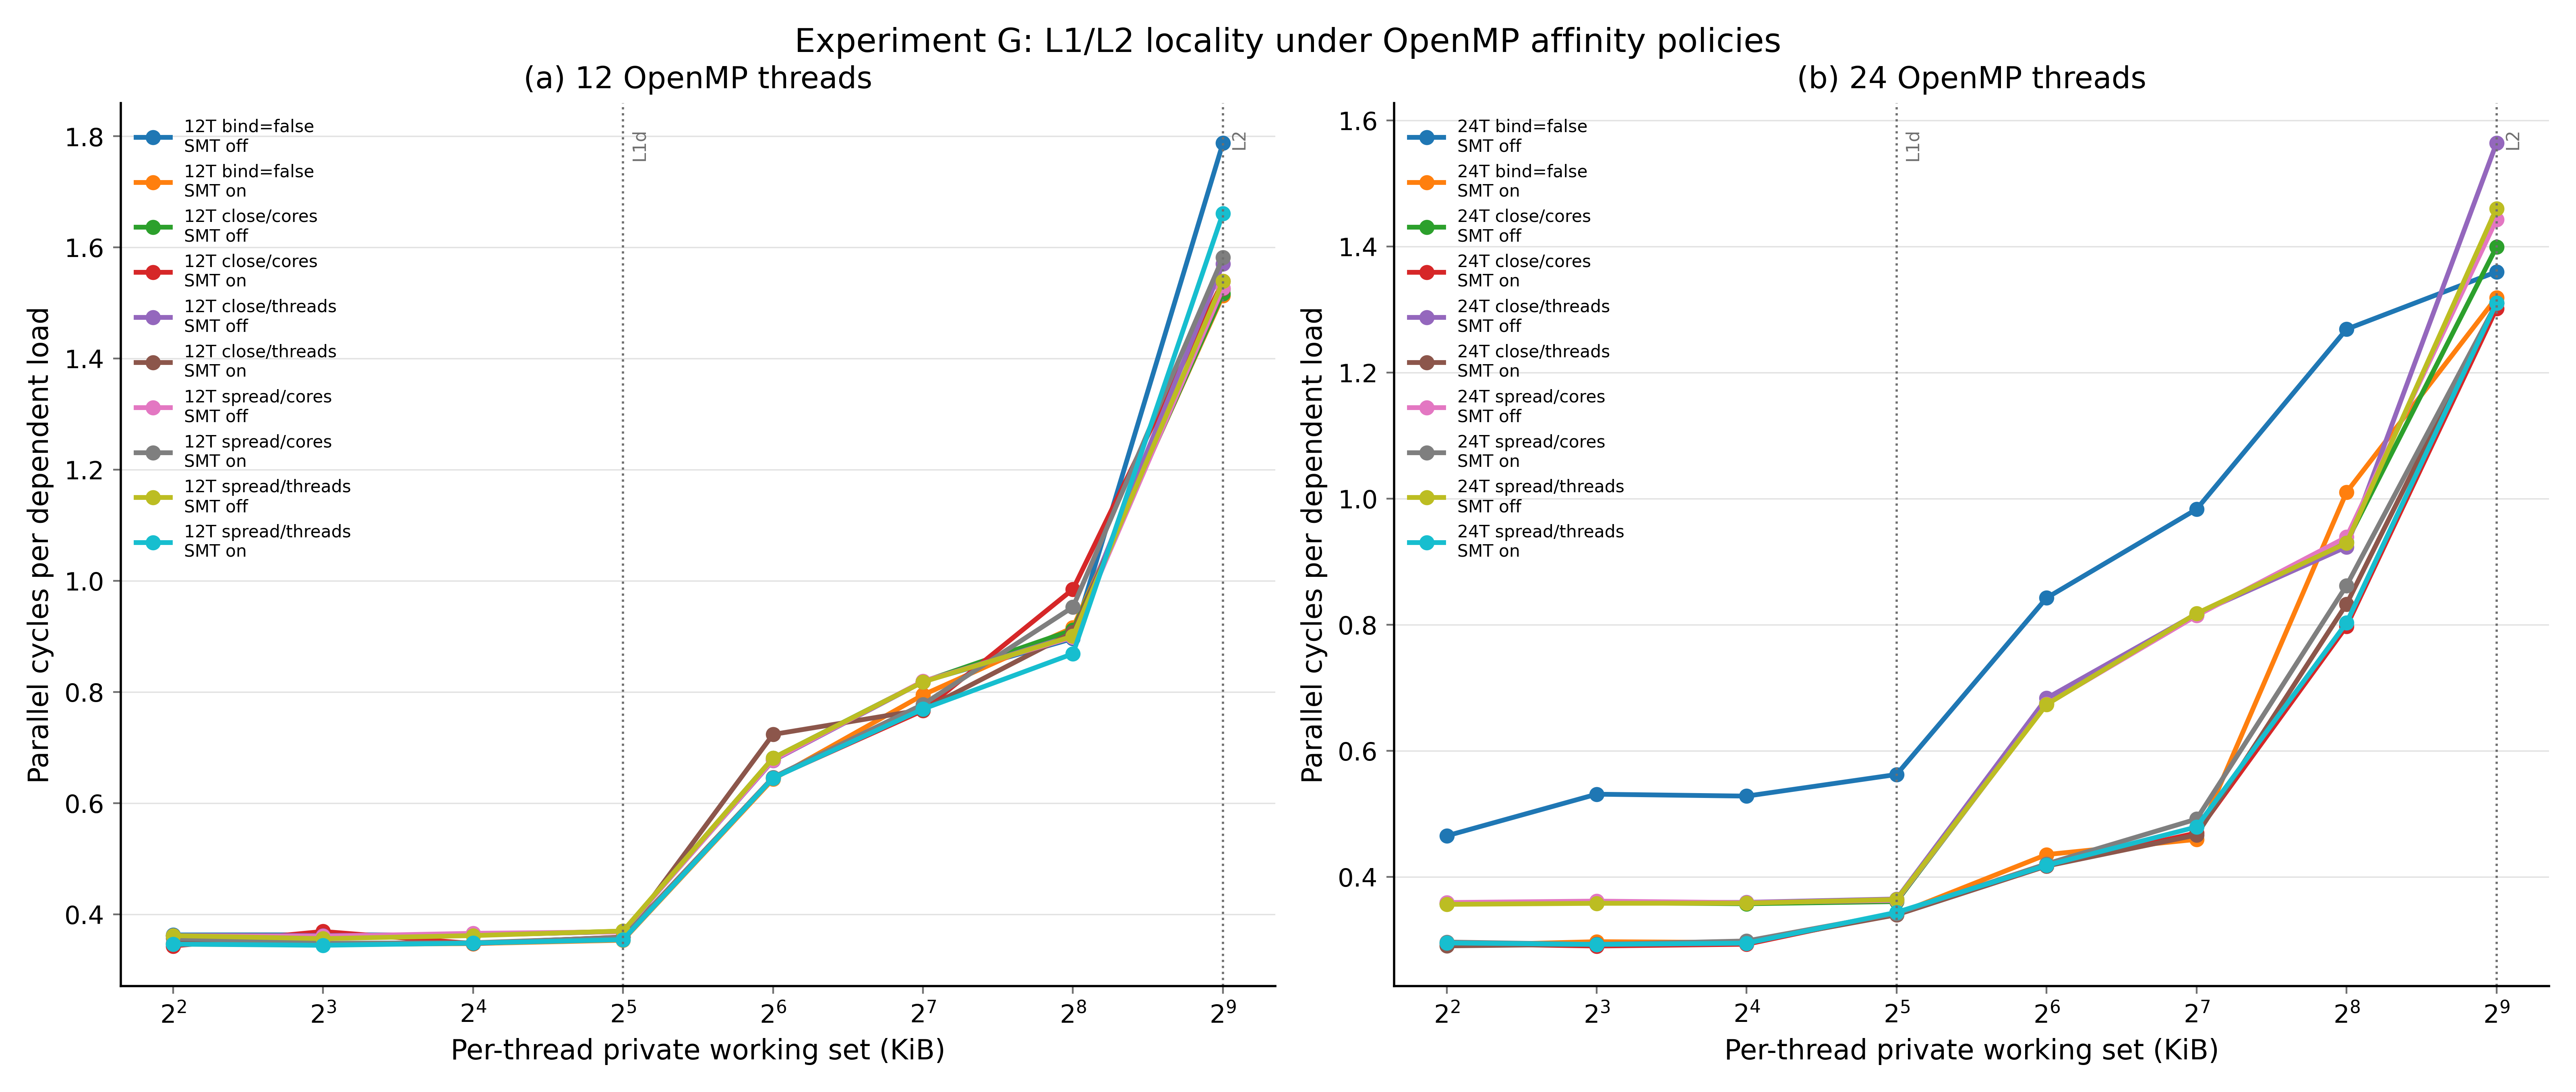
\includegraphics[width=\linewidth]{figure_G_l1_l2_affinity.png}
\caption{실험 G의 OpenMP 스레드 affinity 정책에 따른 L1/L2 캐시 locality 분석 결과.  (a)는 12개의 OpenMP 스레드, (b)는 24개의 OpenMP 스레드를 사용한 환경을 보여준다. 두 그래프 모두 x축은 스레드별 working set 크기를, y축은 병렬 dependent load당 소요 cycle을 나타낸다. 
$2^5$\,KiB (32\,KiB) 및 $2^9$\,KiB (512\,KiB) 부근에 표시된 수직 점선은 각각 L1d와 L2 캐시의 물리적 경계를 의미한다. 모든 조건에서 L1d 캐시 용량을 초과하면서 지연 시간이 점진적으로 증가하는 공통적인 형태를 보이며, 특히 12스레드 환경(a)과 달리 물리 코어 수를 초과하는 24스레드 환경(b)에서는 스레드 고정을 사용하지 않았을 때 지연 시간이 두드러지게 급증하는 등 배치 정책 간의 divergence 확인할 수 있다.}
\label{fig:exp-g-l1-l2-affinity}
\end{figure}

\subsection{Experiment H: Close vs. Spread on Compute-bound Kernel}

그림~\ref{fig:exp-h-bind-compute}는 병렬 for, static 스케줄, 물리 코어 기준 매핑과 활성 대기, 동적 스레드 조절 비활성화를 유지하고 상한은 $10^7$, 사용 가능 CPU는 논리 0--11로 둔 뒤 스레드를 2--6으로 바꾸며 근접 배치와 분산 배치를 비교한 결과이다. 모든 실행에서 실제 OpenMP 스레드 수는 요청값과 동일하게 기록되었다.

SMT-off의 pure speedup은 근접 배치에서 2, 3, 4, 5, 6스레드 순서로 각각 $1.60\times$, $2.29\times$, $2.98\times$, $3.68\times$, $4.38\times$였다. 분산 배치에서는 같은 순서로 $1.59\times$, $2.28\times$, $2.98\times$, $3.68\times$, $4.38\times$가 기록되었다. SMT-off의 6스레드 parallel region time은 근접 배치 2119.36\,ms, 분산 배치 2245.82\,ms였다.

SMT-on의 pure speedup은 근접 배치에서 2, 3, 4, 5, 6스레드 순서로 각각 $1.60\times$, $2.29\times$, $2.97\times$, $3.69\times$, $4.38\times$였다. 분산 배치에서는 같은 순서로 $1.59\times$, $2.28\times$, $2.98\times$, $3.68\times$, $4.38\times$가 기록되었다. SMT-on의 6스레드 parallel region time은 근접 배치 2123.57\,ms, 분산 배치 2248.34\,ms였다.

\begin{figure}[h]
\centering
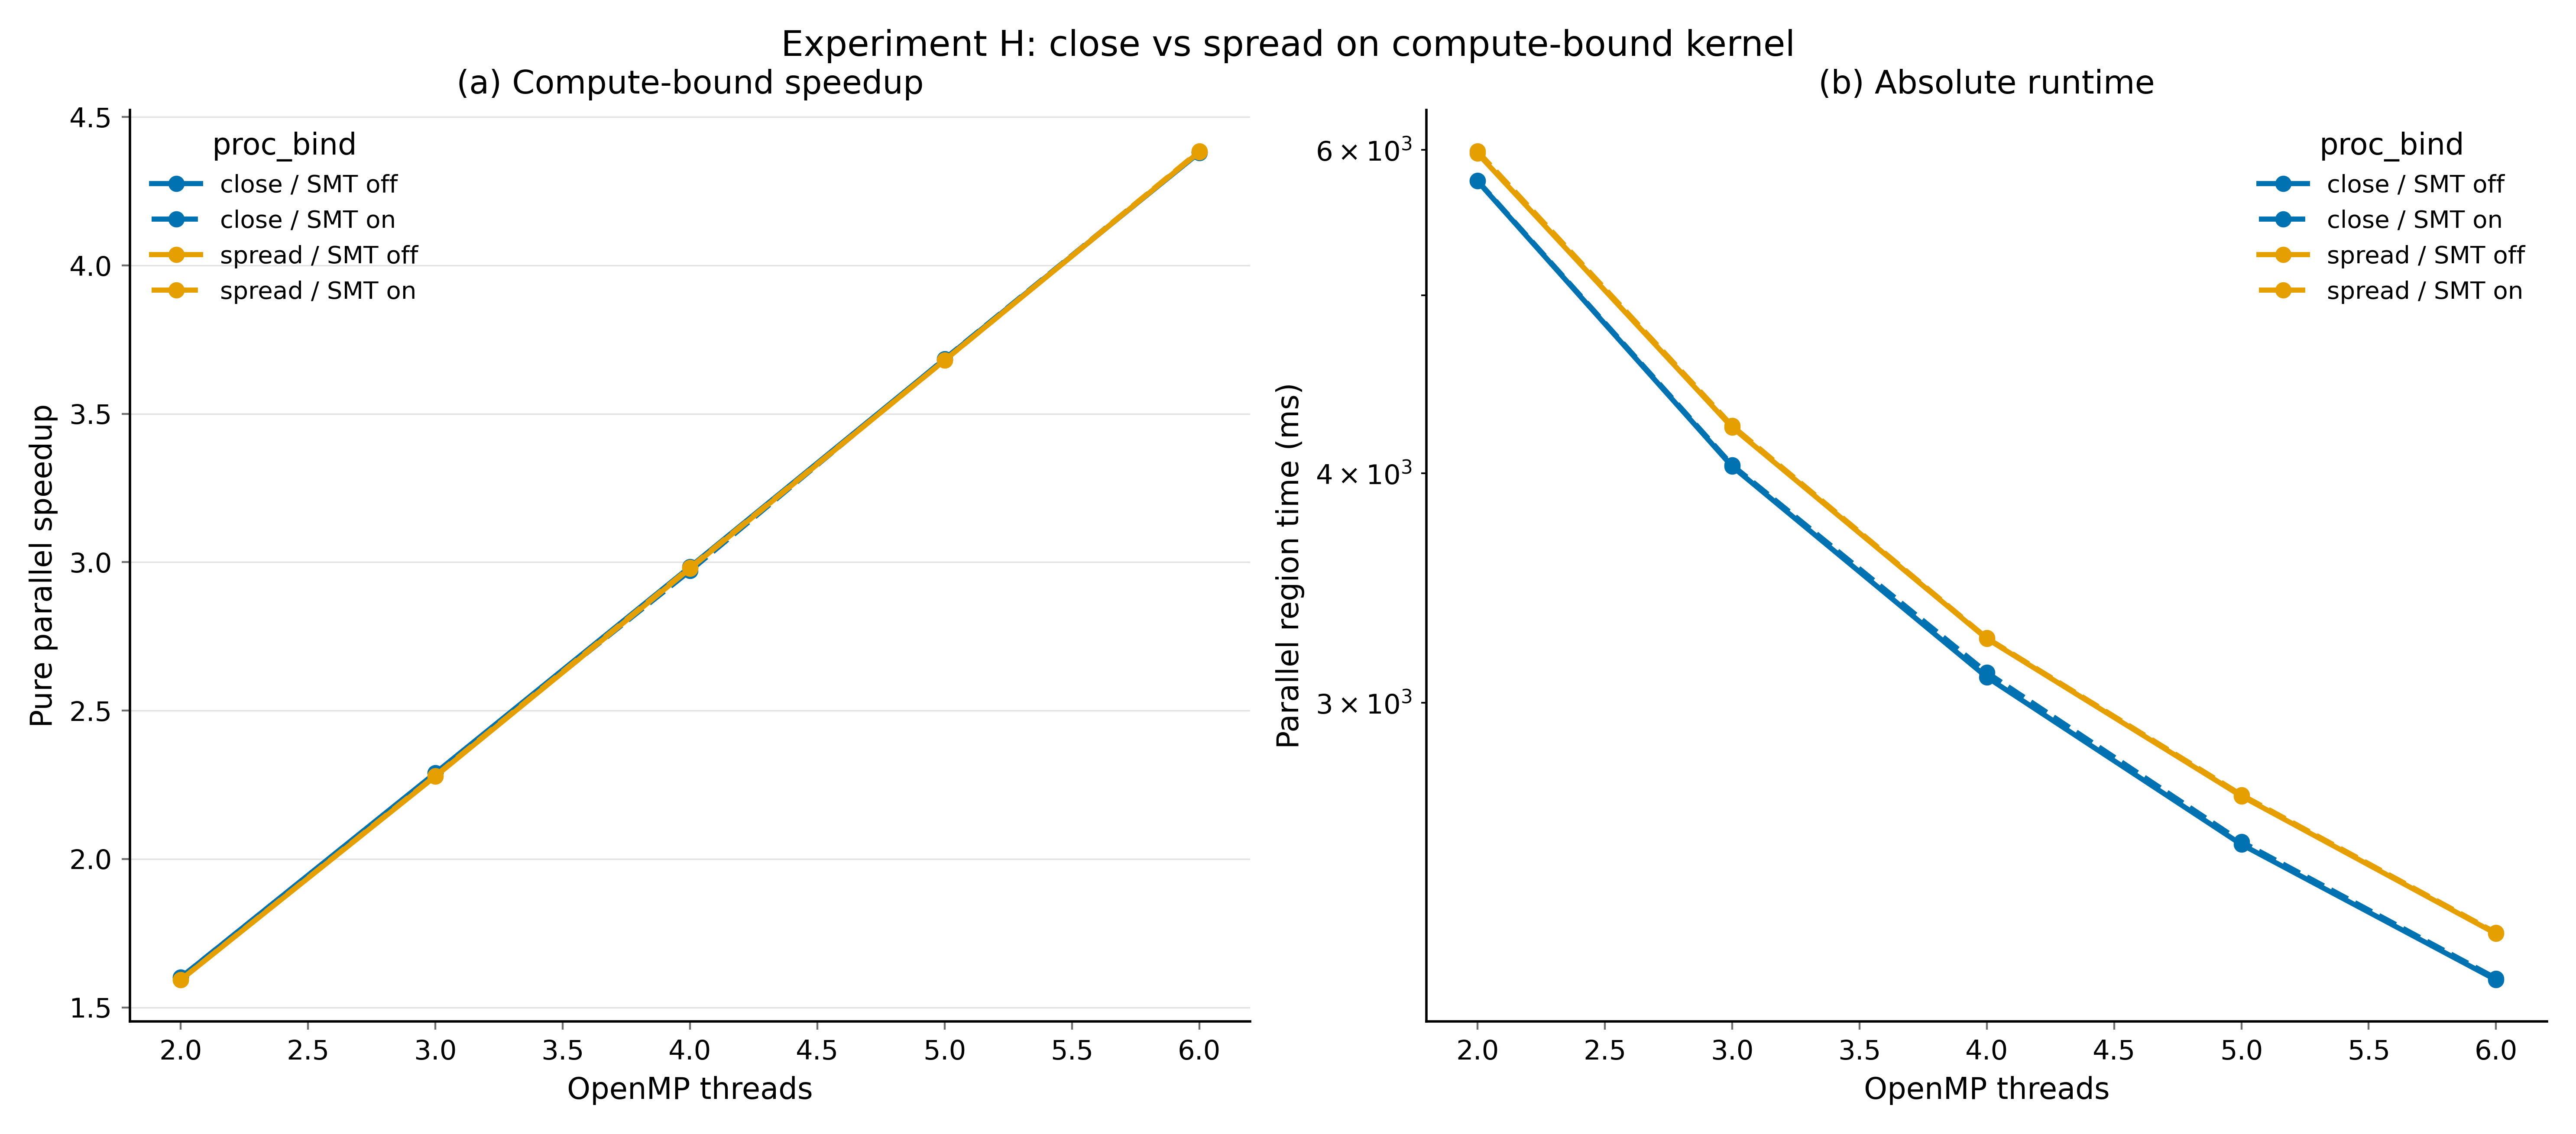
\includegraphics[width=\linewidth]{figure_H_bind_compute.png}
\caption{실험 H의 compute-bound 커널 환경에서 OpenMP 스레드 배치 전략에 따른 성능 비교 결과. (a)는 OpenMP 스레드 수 증가에 따른 pure speedup을 나타내며, (b)는 동일한 스레드 증가에 대한 병렬 영역의 절대 실행 시간을 보여준다. 두 그래프 모두 파란색 선은 스레드를 근접 배치한 경우를, 주황색 선은 분산 배치한 경우를 의미하며, 실선과 점선표식은 각각 SMT-off와 SMT-on 상태를 나타낸다. (a)에서는 스레드 수 증가에 따라 speedup이 선형적으로 증가하며, 조건 간 차이가 거의 드러나지 않는 반면, (b)의 절대 실행 시간 그래프에서는 근접 배치가 분산 배치보다 일관되게 지연 시간이 짧은 것을 확인할 수 있다.}\label{fig:exp-h-bind-compute}
\end{figure}

\subsection{Experiment I: Close vs. Spread on Private Cache Working Sets}

그림~\ref{fig:exp-i-bind-cache}는 스레드별 독립 pointer chase 커널에서
각 스레드의 private working set을 32\,KiB, 512\,KiB,
4096\,KiB로 바꾸고, 스레드를 2--6으로 두며 근접, 분산 배치를 비교한 결과이다. SMT-off와 모든 실행에서 실제 OpenMP 스레드 수는 요청값과 동일하게 기록되었다.

SMT-off의 32\,KiB/thread 조건에서는 dependent load당 cycle이
근접 배치에서 6스레드 기준 $0.640$ cycles/load였고, 분산 배치에서는
$0.674$ cycles/load였다. 같은 조건에서 pure speedup은
근접 배치 $5.94\times$, 분산 배치 $5.90\times$로 기록되었다.
512\,KiB/thread 조건의 6스레드 cycles/load는 근접 배치
$2.882$, 분산 배치 $3.043$였고, 4096\,KiB/thread 조건에서는
근접 배치 $5.894$, 분산 배치 $6.207$ cycles/load였다.

SMT-on의 32\,KiB/thread 조건에서는 6스레드 기준 근접 배치가
$0.775$ cycles/load, 분산 배치가 $1.282$ cycles/load였다.
512\,KiB/thread 조건에서는 근접 배치 $3.256$, 분산 배치
$3.291$ cycles/load였고, 4096\,KiB/thread 조건에서는 근접 배치
$6.163$, 분산 배치 $6.416$ cycles/load였다. 실험 I 전체에서 가장
낮은 cycles/load는 SMT-off의 근접 배치, 6스레드,
32\,KiB/thread 구성에서의 $0.640$ cycles/load였고, SMT-on에서는
근접 배치, 5스레드, 32\,KiB/thread 구성의 $0.769$ cycles/load가
최저값이었다.

\begin{figure}[h]
\centering
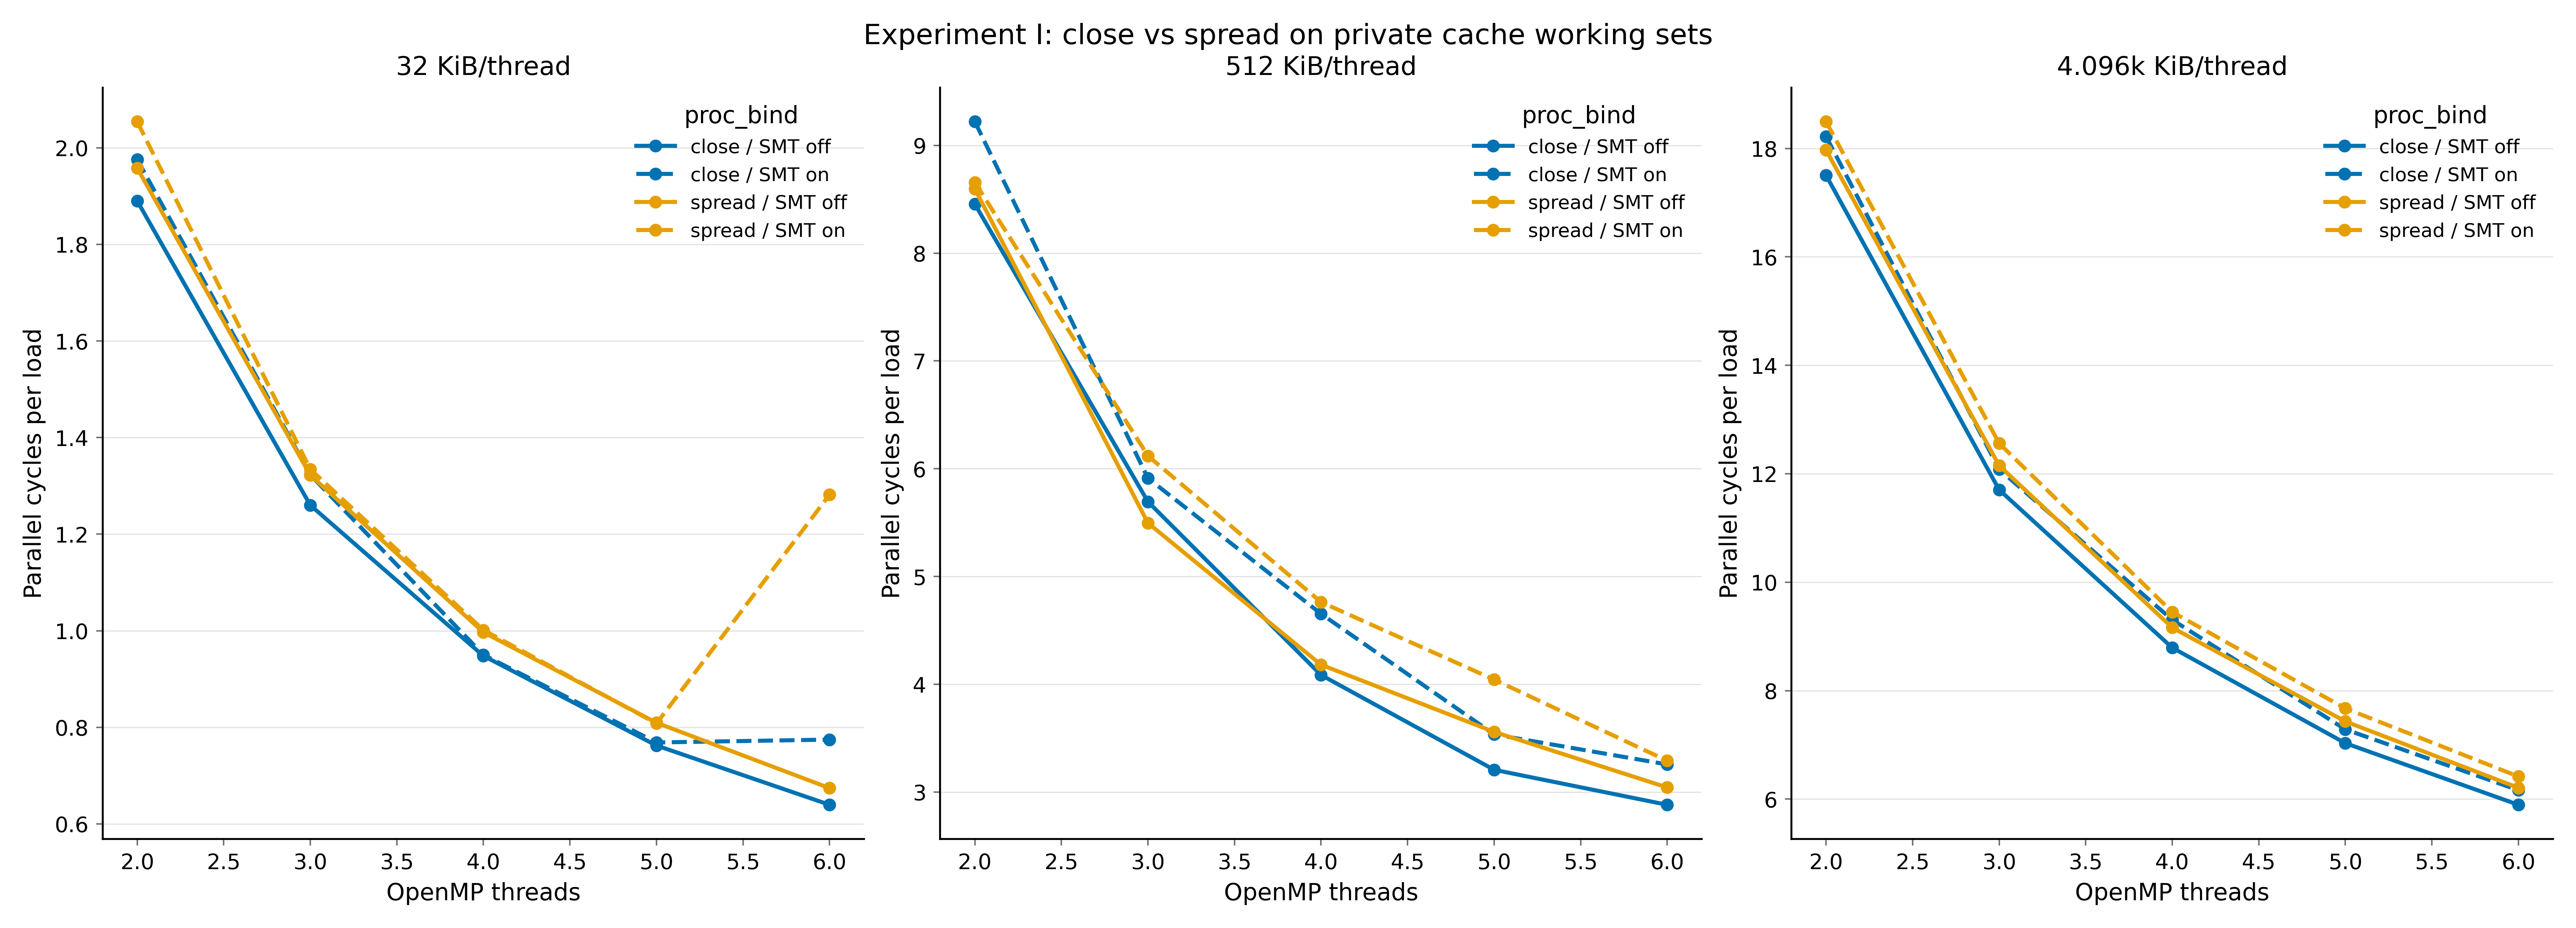
\includegraphics[width=\linewidth]{figure_I_bind_cache.png}
\caption{실험 I의 private 캐시 환경에서 OpenMP 스레드 배치 전략(근접 및 분산)에 따른 성능 비교 결과.  세 개의 그래프는 각각 스레드별 working set 크기에 대한 측정값을 보여준다. 모든 그래프의 x축은 OpenMP 스레드 수(2--6개)를, y축은 병렬 dependent load당 소요 cycle을 나타낸다. 파란색 선은 스레드를 근접 배치한 경우를, 주황색 선은 분산 배치한 경우를 의미하며, 실선과 점선은 각각 SMT-off와 SMT-on 상태를 나타낸다. 스레드 수가 증가함에 따라 지연 시간이 전반적으로 감소하는 경향을 보이며, 모든 working set 크기 조건에서 근접 배치가 분산 배치보다 일관되게 더 낮은 지연 시간을 기록하여 성능상 유리함을 확인할 수 있다.}\label{fig:exp-i-bind-cache}
\end{figure}

\subsection{Experiment J: Intentional False Sharing}

그림~\ref{fig:exp-j-false-sharing}는 공유 라인 버전과 padding 버전 두 커널
(\texttt{false\_sharing}, \texttt{false\_sharing\_padded})을 스레드 수
2, 3, 4, 5, 6, 8, 12, 근접, 분산 배치, 물리 코어 기준 매핑, 활성 대기, 동적 스레드 조절 비활성화,
물리 코어 범위(0--11)로 고정한 뒤 비교한 결과이다. 모든 실행에서 실제 OpenMP 스레드 수는 요청값과 동일하게 기록되었다.

$10^7$에서 근접 배치를 사용한 경우 padded 커널의 cycles/update가 SMT-off에서
2, 3, 4, 5, 6, 8, 12스레드 순서로 $0.519$, $0.412$, $0.274$, $0.224$,
$0.197$, $0.188$, $0.180$ cycles/update였고, SMT-on에서는 $0.512$,
$0.394$, $0.275$, $0.228$, $0.205$, $0.235$, $0.171$ cycles/update였다.
같은 조건의 \texttt{false\_sharing}은 SMT-off에서 $30.226$, $27.422$,
$31.384$, $31.561$, $29.987$, $36.009$, $25.921$ cycles/update였고,
SMT-on에서 $31.625$, $29.450$, $30.309$, $30.854$, $30.425$, $38.446$,
$25.987$ cycles/update였다.

분산 배치에서 $10^7$에서 padding하지 않은 커널은 SMT-off 기준 2스레드 $2.755$ cycles/update,
3스레드 $20.823$ cycles/update, 4--8스레드 $39.695$--$48.479$
cycles/update, 12스레드 $21.992$ cycles/update로 측정되었다. SMT-on에서는
2스레드 $2.777$ cycles/update, 3스레드 $20.365$ cycles/update, 4--8스레드
$41.371$--$43.808$ cycles/update, 12스레드 $26.014$ cycles/update였다.
같은 분산 배치 조건에서 padded 버전 커널은 SMT-off에서
$0.661$에서 $0.126$ cycles/update까지, SMT-on에서 $0.730$에서 $0.132$
cycles/update까지 감소하였다.

실험 J 전체에서 가장 낮은 cycles/update는 SMT-off의
padded 커널, 분산 배치, 12스레드, $10^6$의 $0.124$ cycles/update였고, SMT-on에서는
padded 커널, 분산 배치, 12스레드, $10^7$의 $0.132$ cycles/update였다. 반대로 padding하지 않은 커널의 최대 cycles/update는 SMT-off에서
근접 배치, 2스레드, $10^4$의 $61.237$
cycles/update였고, SMT-on에서는 분산 배치, 4스레드, $10^4$의 $49.289$ cycles/update였다.

\begin{figure}[h]
\centering
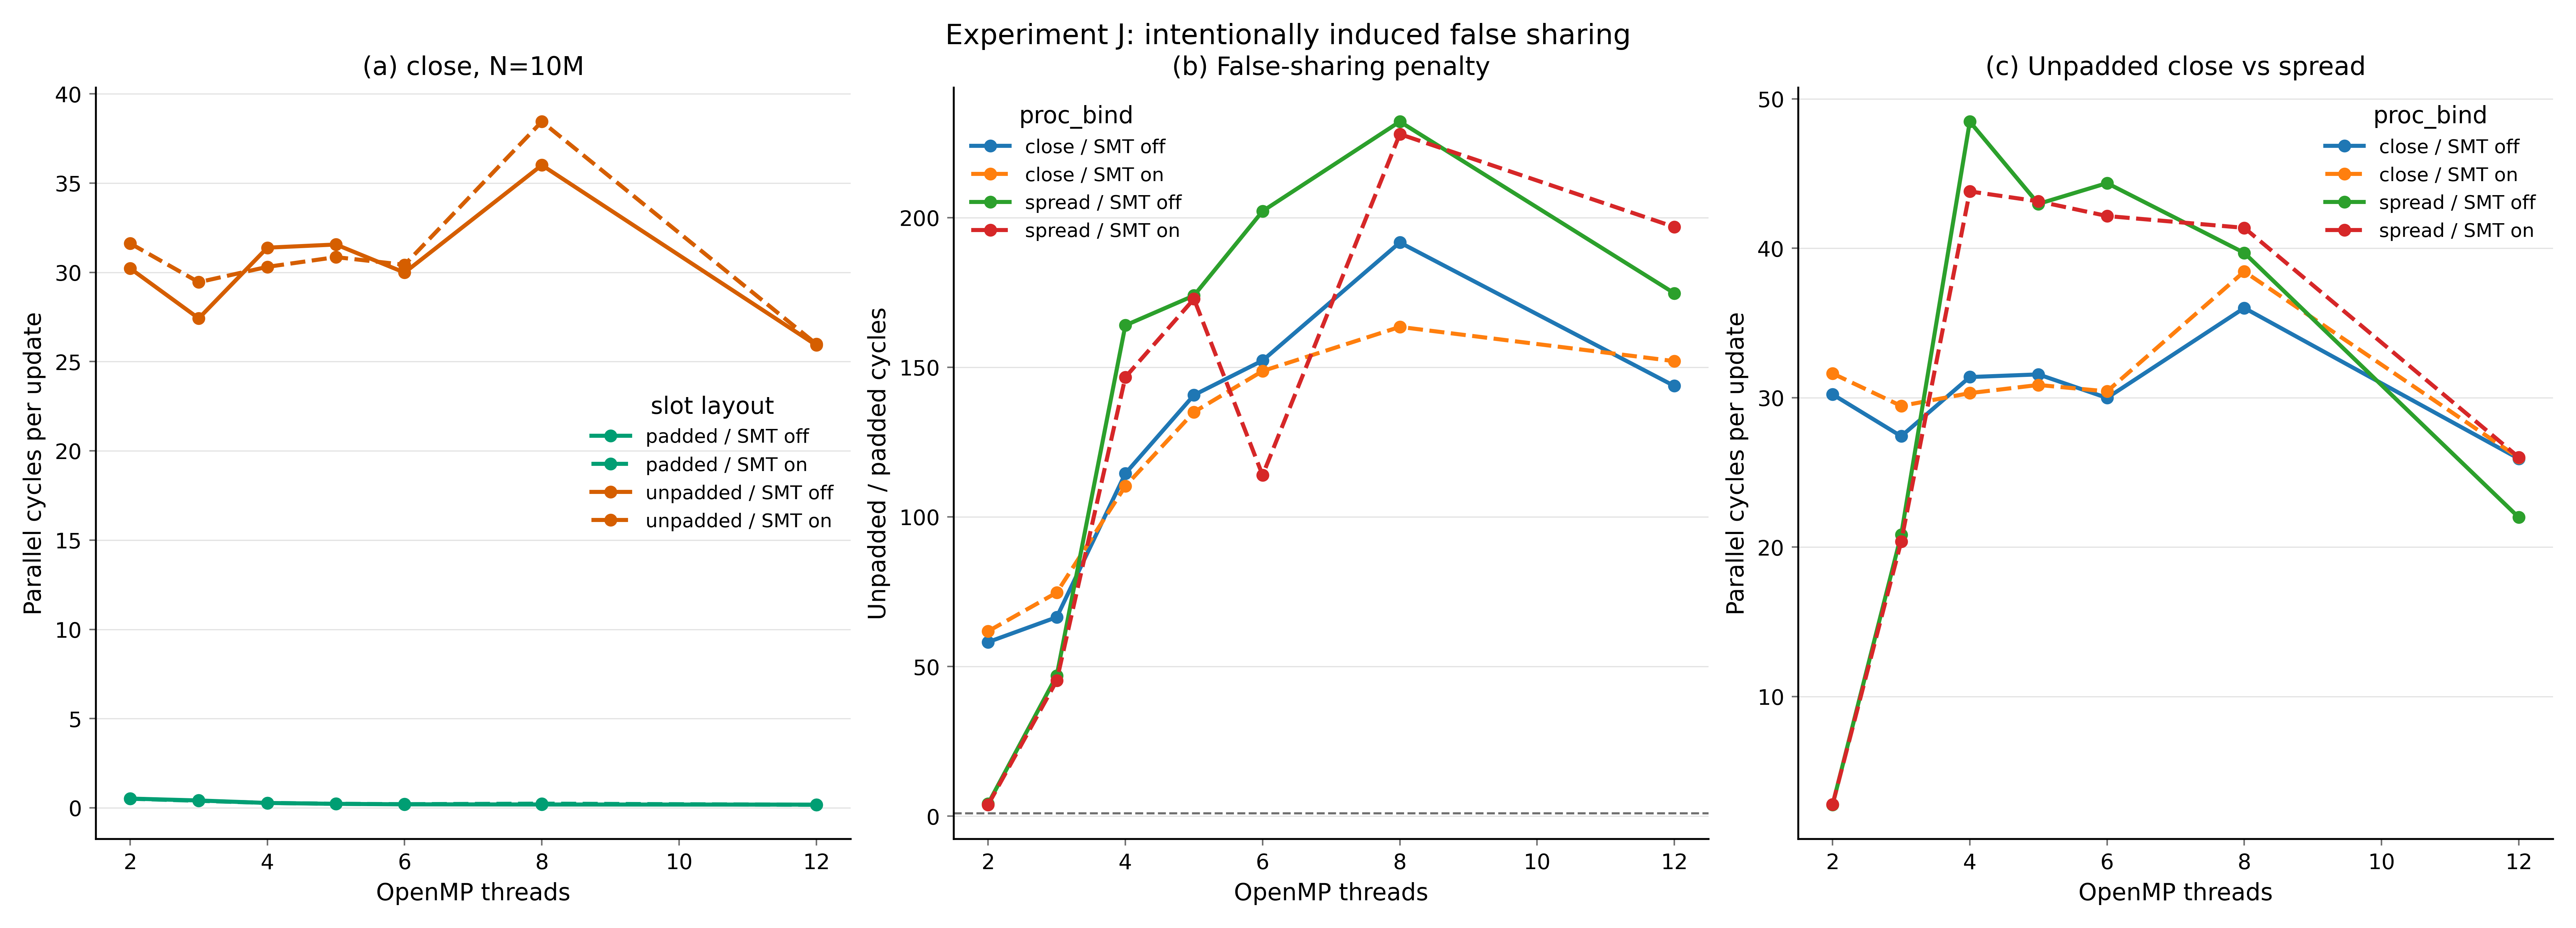
\includegraphics[width=\linewidth]{figure_J_false_sharing.png}
\caption{실험 J의 의도적 false sharing 유발에 따른 성능 저하 및 padding 효과 분석 결과. 
세 개의 그래프 모두 x축은 OpenMP 스레드 수(2--12)를 나타낸다. 
(a)는 근접 배치 조건에서 병렬 갱신당 소요 cycle을 보여주며, 캐시 라인을 공유하는 비패딩 조건이 간격을 128\,B로 벌린 패딩 조건에 비해 지연 시간이 극단적으로 치솟는 것을 대조적으로 보여준다. 
(b)는 패딩 적용 대비 미적용 시의 latency 비율을 나타낸 그래프로, 스레드 배치 전략과 스레드 수 증가에 따라 성능 저하 배율이 최대 수백 배까지 요동치는 양상을 시각화한다. 
(c)는 비패딩 조건에 한정하여 latency를 근접 배치와 분산 배치 간에 직접 비교한 그래프이다. 
모든 그래프에서 실선과 점선은 각각 SMT-off와 SMT-on 상태를 의미하며, 다중 스레드 환경에서 단일 캐시 라인 공유가 야기하는 극심한 성능 병목 현상과 메모리 패딩을 통한 해결을 확인 가능하다.}\label{fig:exp-j-false-sharing}
\end{figure}

\section{Analysis}

본 실험의 결과는 naive prime search의 병렬 성능이 단순히 사용한 스레드 수에 의해 결정되지 않고, 반복 공간의 부하 불균형, OpenMP 런타임의 작업 분배 방식, 스레드 배치/고정, 그리고 캐시 계층의 경계가 함께 작용한 결과임을 보여준다. 특히 계산 중심 실험과 메모리 중심 실험은 서로 다른 병목을 드러냈다. naive prime search 커널에서는 정수의 크기가 커질수록 trial division 반복 횟수가 증가하기에, 같은 반복 한 번이라도 뒤쪽
구간의 계산 비용이 더 크다. 반면 pointer chase 및 false sharing 실험에서는 산술 연산보다 캐시 hit/miss, CCD 경계, coherence traffic이 성능을 지배하였다.

\subsection{계산 중심 커널의 확장성과 부하 불균형}

실험 A의 strong scaling 결과에서 $10^7$ 입력 기준 12스레드는 SMT-off와 SMT-on 모두 약 $8.6\times$의 pure speedup을 기록하였다. 이는 naive prime search가 충분히 큰 입력에서는 병렬화 이득을 얻지만, 12개 물리 코어에 대해 선형적인 성능 향상인 $12\times$까지는 도달하지 못하였다. 주된 이유는 두 가지로 판단된다. 첫째, 작은 \texttt{limit}에서는 병렬 영역 진입, fork--join, scheduling 비용이 계산 시간에 비해
커서 스레드 증가가 안정적인 이득으로 이어지지 않는다. 실제로 일부 작은 입력에서 더 높은 pure speedup이 관찰되었다. 하지만, 이는 계산 시간이 짧아 오차가 크기에 결과를 신뢰하기는 어렵다. 둘째, 큰 입력에서도 \texttt{static, chunk=0}으로 연속 구간을 분배하면 후보값이 큰 뒤쪽 구간을 맡은 스레드가 더 오래 실행되어 load imbalance가 발생한다.

이는 실험 B에서 확인된다. 동일한 12스레드, $10^7$ 입력 조건에서 \texttt{static, chunk=0}은 약 $8.6\times$에 머물렀지만, \texttt{guided} 또는 적절한 \texttt{dynamic} chunk를 사용하면 SMT-off에서 최대 $12.43\times$, SMT-on에서 최대 $11.98\times$까지, 즉, 사실상 선형적인 성능 향상에 가깝게 나타났다. 즉, naive prime search의 병목은 병렬화 자체의 한계라기보다 반복별 계산량이 균일하지 않은 상태에서 정적 작업 분배 방식을 사용한 것에서 크게 발생하는 것이다. \texttt{guided}는 초반에는 큰 chunk로 scheduling overhead를 줄이고, 후반에는 작은 chunk로 남은 고비용 반복을 여러 스레드에 분산하므로 이 커널의 비용 구조와 잘 맞았다.  반대로 \texttt{static, chunk=1}이나 작은 \texttt{task\_chunk\_size}는 부하 균형에는 유리할 수 있지만, 반복마다 runtime queue 또는 task 관리 비용이 커져 pure speedup이 크게
낮아졌다. 따라서 본 과제의 계산 커널처럼 불균형이 심할 것이라고 예상되는 때에서는 ``작업을 얼마나 많이 나누는가''보다
``불균형을 줄일 만큼만 나누고, runtime overhead를 억제하는가''가 더 중요한 조건임을 확인하였다.

\subsection{SMT, 스레드 배치/고정, CCD 배치의 영향}

SMT의 효과는 커널 종류에 따라 다르게 나타났다. 계산 중심 실험에서 12개 물리 코어를 사용하는 경우 SMT-off와 SMT-on의 차이는 작았다. 실험 A의 $10^7$ 기준 12스레드 pure speedup은 두 모드 모두 약 $8.6\times$였고, 실험 H에서도 2--6스레드 구간의 근접, 분산 배치 결과가 거의 동일했다. 이는 해당 naive prime search 커널이 추가 SMT sibling을 적극적으로 활용할 만큼 latency hiding 여지가 크지 않고, 이미 물리 코어 단위의 integer 연산이 주요하기 때문이라고 해석할 수 있다. SMT-on의 24스레드가 12스레드 대비 큰 추가 이득을 만들지 못한 것도 같은 맥락이라 판단된다. 하나의 물리 코어에서 두 논리 스레드가 front-end, execution unit, L1/L2를 공유하므로, 독립적인 물리 코어를 추가하는 것과 같은 효과를 기대하기 어렵다.

스레드 배치/고정은 성능을 크게 개선하기보다는 잘못된 배치를 피하는 control variable로만 작용하였다. 실험 C에서 SMT-off의 물리 코어 단위 분산 배치가 가장 높았지만 물리 코어 단위 근접 배치와의 차이는 크지 않았다. 12개 스레드를 모두 사용하면 어차피 두 CCD의 모든 물리 코어를 사용하므로, 두 고정 방식 간 차이가 작아지는 것이 자연스럽다. 반면 SMT-on에서 논리 스레드 단위 근접 배치가 $4.41\times$로 크게 낮아진 결과는 예상치 못하였다. 논리 스레드 단위 매핑에서 근접 배치가 논리 코어를 인접하게 채우면 일부 물리 코어의 SMT 형제 스레드를 먼저 사용하거나 배치가 한쪽으로 치우칠 수 있고, 이 경우 물리 코어 전체를 고르게 쓰는 구성보다 자원 경합이 커진다. 따라서 SMT-on 환경에서는 단순히 스레드 수만 맞추는 것이 아니라, 배치 대상 단위 선택과 근접, 분산 정책을 실제 CPU topology와 함께 고려해야 한다.

실험 D에서 동적 스레드 수 조절을 켠 경우도 위 결론을 뒷받침한다. 런타임이 실제 스레드 수를 8--9개로 줄이면서 $10^7$ 입력의 pure speedup은 고정 12스레드보다 낮아졌다. 일반적인 runtime heuristic은 시스템 전체 부하나 내부 정책을 바탕으로 스레드 수를 조절하지만,
본 실험처럼 고정된 계산 커널에서 물리 코어 수와 스레드 배치/고정을 명시적으로 통제한 경우에는 자동 조정이 오히려 실험 의도와 어긋날 수 있다. 따라서 성능 비교를 목적으로 하는 OpenMP 실험에서는 동적 스레드 수 조절을 끈 뒤 실제 스레드 수를 고정하고, 스레드 대기 정책은 짧은 병렬 영역의 fork--join 비용과 긴 계산 구간의 wall time을 함께 보며 선택해야 함을 알 수 있다.

\subsection{캐시 계층과 Coherence 비용}

캐시 실험은 Ryzen Zen 3의 계층 구조가 결과에 직접적인 영향을 끼친다. 실험 E에서 단일 스레드 pointer chase는 4--32\,KiB 구간에서 약 $3.8$ cycles/load로 낮게 유지되었고, 64\,KiB부터 지연 시간이 증가하기 시작하였다. 이는 L1D 32\,KiB 경계를 넘어 L2 접근이 섞이기 시작한 결과로 해석할 수 있다. 512\,KiB와 1\,MiB에서 각각 더 큰 증가가 나타난
것은 L2 용량 경계의 영향이며, 32\,MiB 이후와 64--128\,MiB 구간의 급격한 증가는 CCD 내 L3 용량을 넘어 DRAM에 접근이 필요한 영역으로 넘어간 결과이다. pointer chase는 다음 주소가 이전 load 결과에 의존하기에 하드웨어 prefetcher와 memory-level parallelism의 도움을 거의 받지 못한다. 따라서 이 실험의 cycles/load는 일반 스트리밍 bandwidth보다 cache latency 계층을 더 직접적으로 반영한다.

실험 F의 CCD 배치 비교에서는 4--32\,MiB 구간에서 단일 CCD 배치와 CCD 분할 배치 사이의 차이가 작지만 관찰되었고, 64\,MiB 이상에서는 단일 배치와 분할 배치 모두 비슷하게 좋지 않은 결과를 보였다. 이는 working set이 한 CCD의 32\,MiB L3 안에 들어가거나 근접한 구간에서는 배치와 L3 공유 여부가 영향을 줄 수 있지만, working set이 64\,MiB 이상으로 커지면 두 CCD의 L3를 합친 용량도 넘어서거나 DRAM 접근 비중이 커져 스레드 배치 효과가 상대적으로 작아지기 때문이다. 실험 I에서도 private working set이 32\,KiB일 때는 근접 배치가 분산 배치보다 낮은 cycles/load를 보였으며, 512\,KiB 및 4096\,KiB로 커질수록 절대 비용이 증가하였다. 이는 스레드별 working set이 L1/L2에 들어갈 때에는 같은 물리 코어에 안정적으로 고정되는 것이 중요하지만, working set이 private cache를
넘어서면 L3 및 메모리 계층의 영향이 커진다는 점을 보여준다.

false sharing 실험은 캐시 용량 문제가 아니더라도 캐시 라인 단위 coherence가 병렬
성능을 압도할 수 있음을 가장 명확하게 보여준다. 실험 J에서 padding을 적용한 구성은
$0.12$--$0.13$ cycles/update 수준까지 낮아졌지만, 같은 64\,B 캐시 라인을 여러
스레드가 갱신한 구성은 수십 cycles/update까지 악화되었다. 두 구현은 반복 횟수와
스레드 수가 같고, 차이는 스레드별 저장 위치가 같은 캐시 라인에 놓이는지 여부뿐이다.
따라서 성능 차이는 계산량이 아니라 cache line ownership이 스레드 사이에서 반복적으로
이동하는 coherence traffic에서 비롯된다. 이는 OpenMP 병렬화에서 스레드별 accumulator,
통계 배열, per-thread buffer를 설계할 때 cache line padding 또는 alignment가 실제
성능에 결정적인 영향을 줄 수 있음을 의미한다.

\subsection{종합 해석}

전체 결과를 종합하면, 본 과제의 최적화 방향은 커널의 병목에 따라 달라진다. 계산 중심 naive prime search에서는 SMT 사용 여부보다 반복 공간의 부하 불균형을 줄이는 scheduling 정책이 더 큰 영향을 주었다. 특히 \texttt{guided} 및 적절한 \texttt{dynamic} chunk는 \texttt{static, chunk=0} 대비 큰 성능 향상을 만들었다. 반면 캐시 및 coherence 중심 커널에서는 스케줄링보다 working set 크기, 스레드 배치/고정, CCD 배치, cache line 공유 여부가 결과를 지배하였다. 즉, OpenMP에서도 no free lunch theorem이 적용된다는 것을 확인할 수 있었다. 계산 불균형이 큰 커널에서는 동적 작업 분배 방식을, private cache locality가 중요한 커널에서는 안정적인 스레드 배치 및 고정을, false sharing이 예상되는 커널에서는 cache line 단위의 데이터 배치를 고려하는 것이 필요하다.

또한 본 실험은 SMT-on이 항상 빠르거나 SMT-off가 항상 안정적이라는 단순한 결론으로 환원되지 않는다. SMT-on은 24스레드 private cache 실험처럼 일부 latency-bound 조건에서 낮은 cycles/load를 보일 수 있었지만, 계산 중심 naive prime search에서는 물리 코어 12개를 넘는 확장이 제한적이었다. SMT-off는 물리 코어와 OpenMP 스레드의 대응이 단순하여 해석과 재현성이 좋았고, 물리, 논리 스레드 단위 place 선택에 따른 예외적 배치 위험도 작았지만, 병목 구간에서 파이프라인 유휴 자원을 활용하지 못해 latency-bound 조건에서는 오히려 자원 활용도가 떨어지는 약점을 보였다.

\section{Limitations}

본 실험은 AMD Ryzen 9 5900X (Zen 3) 단일 시스템에서만 수행되었다. 실험 결과는 Zen 3 특유의 6코어 단위 CCD 구조와 32\,MiB 단위의 L3 캐시 공유 구조에 기반하기에, P-Core와 E-Core를 혼용하는 비대칭 아키텍처나 캐시 계층 구조 및 shvar 관리 메커니즘이 근본적으로 다른 타 ISA에서는 본 보고서의 결과/결론과 다른 양상이 나타날 수 있다.

또한, 실험에 사용된 커널은 계산 중심의 naive prime search와 메모리 부하를 유도하기 위해 합성된 pointer chase, 의도적 false sharing 커널 등 특정 작업에서의 동작 및 결과만을 관찰하기 위해 설계되었다. 즉, 실제 일반적인 환경 및 애플리케이션에서의 동작과 결과가 다르게 나올 수 있다.

이에 더해, os interrupt나 백그라운드 작업에 의한 노이즈를 최소화하고자 하였다. 다만, os위에서 진행한 실험으로 커널 스케줄러의 개입 등으로 인한 지연 오차를 근본적으로 제어가 불가능하다. 특히, 수행 시간이 수 ms로 짧은 결과들의 경우, 해당 결과에 대한 신뢰가 어렵다.

\section*{Acknowledgement}
본 보고서에서 사용 및 활용된 코드들의 작성 및 보고서 용어 통일 및 수정은 Claude 4.7 Opus 및 OpenAI GPT 5.5가 수행하였습니다. 단, 코드 구조 설계, 실험 설계, 결과 해석, 보고서 작성은 작성자 본인이 직접 수행하였음을 명확하게 밝힙니다.

\clearpage
\appendix
\section{Configuration Files}
\label{app:configs}

본 appendix는 실험별 grid search에 사용한 search space 정의 및 설정 파일의 전문을 수록한다.

\subsection{\texttt{search\_space.yaml}}
\lstinputlisting[basicstyle=\ttfamily\scriptsize]{../configs/search_space.yaml}

\subsection{\texttt{search\_space\_A\_scaling.yaml}}
\lstinputlisting[basicstyle=\ttfamily\scriptsize]{../configs/search_space_A_scaling.yaml}

\subsection{\texttt{search\_space\_B\_schedule.yaml}}
\lstinputlisting[basicstyle=\ttfamily\scriptsize]{../configs/search_space_B_schedule.yaml}

\subsection{\texttt{search\_space\_C\_affinity.yaml}}
\lstinputlisting[basicstyle=\ttfamily\scriptsize]{../configs/search_space_C_affinity.yaml}

\subsection{\texttt{search\_space\_D\_runtime.yaml}}
\lstinputlisting[basicstyle=\ttfamily\scriptsize]{../configs/search_space_D_runtime.yaml}

\subsection{\texttt{search\_space\_E\_cache.yaml}}
\lstinputlisting[basicstyle=\ttfamily\scriptsize]{../configs/search_space_E_cache.yaml}

\subsection{\texttt{search\_space\_F\_l3\_ccd.yaml}}
\lstinputlisting[basicstyle=\ttfamily\scriptsize]{../configs/search_space_F_l3_ccd.yaml}

\subsection{\texttt{search\_space\_G\_l1\_l2\_affinity.yaml}}
\lstinputlisting[basicstyle=\ttfamily\scriptsize]{../configs/search_space_G_l1_l2_affinity.yaml}

\subsection{\texttt{search\_space\_H\_bind\_compute.yaml}}
\lstinputlisting[basicstyle=\ttfamily\scriptsize]{../configs/search_space_H_bind_compute.yaml}

\subsection{\texttt{search\_space\_I\_bind\_cache.yaml}}
\lstinputlisting[basicstyle=\ttfamily\scriptsize]{../configs/search_space_I_bind_cache.yaml}

\subsection{\texttt{search\_space\_J\_false\_sharing.yaml}}
\lstinputlisting[basicstyle=\ttfamily\scriptsize]{../configs/search_space_J_false_sharing.yaml}

\section{Code Listings}
\label{app:code}

본 Appendix에서는 실험에 사용한 주요 코드들의 주요 클래스 및 함수를 수록한다.

\subsection{\texttt{main.c}}
\label{app:code-main}

\subsection{\texttt{run\_experiments.py}}

\subsection{\texttt{grid\_search.py}}

\begin{thebibliography}{9}

\bibitem{amd-ppr-family19h}
Advanced Micro Devices, Inc.,
\emph{Processor Programming Reference (PPR) for AMD Family 19h Processors},
pp. 81--84,
AMD Technical Documentation.
\url{https://docs.amd.com/api/khub/documents/pl6ZFPOSOcLQBUlgPjv3jw/content?Ft-Calling-App=ft\%2Fturnkey-portal\&Ft-Calling-App-Version=5.3.1}
(accessed 2026-04-27).

\end{thebibliography}

\end{document}
